%%%%%%%%%%%%%%%%%%%%%%%%%%%%%%%%%%%%%%%%%%%%%%%%%%%%%%%%%%%%%%%%%%%%%%%%%%%%
% AGUJournalTemplate.tex: this template file is for articles formatted with LaTeX
%
% This file includes commands and instructions
% given in the order necessary to produce a final output that will
% satisfy AGU requirements, including customized APA reference formatting.
%
% You may copy this file and give it your
% article name, and enter your text.
%
%
% Step 1: Set the \documentclass
%
%

%% To submit your paper:
\documentclass[draft]{agujournal2019}
\usepackage{url} %this package should fix any errors with URLs in refs.
\usepackage{lineno}
\usepackage[inline]{trackchanges} %for better track changes. finalnew option will compile document with changes incorporated.
\usepackage{soul}
\linenumbers
\usepackage{graphicx}
\usepackage{subcaption}
\usepackage{amsmath,amsfonts,amsthm,bm}
\usepackage{amssymb}
\usepackage[fleqn,tbtags]{mathtools}
\usepackage{tensor}
\usepackage{microtype}
\usepackage{breakcites}
\usepackage{siunitx}
\usepackage{multirow}
\usepackage{xcolor}
\usepackage[geometry]{ifsym}
%%%%%%%
% As of 2018 we recommend use of the TrackChanges package to mark revisions.
% The trackchanges package adds five new LaTeX commands:
%
%  \note[editor]{The note}
%  \annote[editor]{Text to annotate}{The note}
%  \add[editor]{Text to add}
%  \remove[editor]{Text to remove}
%  \change[editor]{Text to remove}{Text to add}
%
% complete documentation is here: http://trackchanges.sourceforge.net/
%%%%%%%

\draftfalse

%% Enter journal name below.
%% Choose from this list of Journals:
%
% JGR: Atmospheres
% JGR: Biogeosciences
% JGR: Earth Surface
% JGR: Oceans
% JGR: Planets
% JGR: Solid Earth
% JGR: Space Physics
% Global Biogeochemical Cycles
% Geophysical Research Letters
% Paleoceanography and Paleoclimatology
% Radio Science
% Reviews of Geophysics
% Tectonics
% Space Weather
% Water Resources Research
% Geochemistry, Geophysics, Geosystems
% Journal of Advances in Modeling Earth Systems (JAMES)
% Earth's Future
% Earth and Space Science
% Geohealth
%
% ie, \journalname{Water Resources Research}

\journalname{Enter journal name here}


\begin{document}

%% ------------------------------------------------------------------------ %%
%  Title
%
% (A title should be specific, informative, and brief. Use
% abbreviations only if they are defined in the abstract. Titles that
% start with general keywords then specific terms are optimized in
% searches)
%
%% ------------------------------------------------------------------------ %%

\title{Seismic response associated with the poroelastic effects from an isolated fracture-damage zone system}

% \title{Poroelastic effects of the damage zone on fracture normal compliance and reflectivity}

%% ------------------------------------------------------------------------ %%
%
%  AUTHORS AND AFFILIATIONS
%
%% ------------------------------------------------------------------------ %%

% Authors are individuals who have significantly contributed to the
% research and preparation of the article. Group authors are allowed, if
% each author in the group is separately identified in an appendix.)

% List authors by first name or initial followed by last name and
% separated by commas. Use \affil{} to number affiliations, and
% \thanks{} for author notes.
% Additional author notes should be indicated with \thanks{} (for
% example, for current addresses).

% Example: \authors{A. B. Author\affil{1}\thanks{Current address, Antartica}, B. C. Author\affil{2,3}, and D. E.
% Author\affil{3,4}\thanks{Also funded by Monsanto.}}

\authors{=list all authors here=}


% \affiliation{1}{First Affiliation}
% \affiliation{2}{Second Affiliation}
% \affiliation{3}{Third Affiliation}
% \affiliation{4}{Fourth Affiliation}

\affiliation{=number=}{=Affiliation Address=}
%(repeat as many times as is necessary)

%% Corresponding Author:
% Corresponding author mailing address and e-mail address:

% (include name and email addresses of the corresponding author.  More
% than one corresponding author is allowed in this LaTeX file and for
% publication; but only one corresponding author is allowed in our
% editorial system.)

% Example: \correspondingauthor{First and Last Name}{email@address.edu}

\correspondingauthor{=name=}{=email address=}

%% Keypoints, final entry on title page.

%  List up to three key points (at least one is required)
%  Key Points summarize the main points and conclusions of the article
%  Each must be 100 characters or less with no special characters or punctuation and must be complete sentences

% Example:
% \begin{keypoints}
% \item	List up to three key points (at least one is required)
% \item	Key Points summarize the main points and conclusions of the article
% \item	Each must be 100 characters or less with no special characters or punctuation and must be complete sentences
% \end{keypoints}

\begin{keypoints}
\item enter point 1 here
\item enter point 2 here
\item enter point 3 here
\end{keypoints}

%% ------------------------------------------------------------------------ %%
%
%  ABSTRACT and PLAIN LANGUAGE SUMMARY
%
% A good Abstract will begin with a short description of the problem
% being addressed, briefly describe the new data or analyses, then
% briefly states the main conclusion(s) and how they are supported and
% uncertainties.

% The Plain Language Summary should be written for a broad audience,
% including journalists and the science-interested public, that will not have 
% a background in your field.
%
% A Plain Language Summary is required in GRL, JGR: Planets, JGR: Biogeosciences,
% JGR: Oceans, G-Cubed, Reviews of Geophysics, and JAMES.
% see http://sharingscience.agu.org/creating-plain-language-summary/)
%
%% ------------------------------------------------------------------------ %%

%% \begin{abstract} starts the second page

\begin{abstract}
Fluid pressure diffusion (FPD) between a fracture and a porous permeable background can increase the normal compliance of the fracture and thus its reflectivity. However, many fractured reservoirs of interest are associated with largely impermeable background rocks acting as flow barriers. Nonetheless, there is evidence to suggest that the seemingly ubiquitous presence of damaged zones (DZ) around fractures can provide the necessary hydraulic communication for FPD to occur between fractures and their surroundings. We investigate FPD effects on fracture reflectivity and normal compliance related to the presence of a DZ.
%embedded in a impermeable background.
To this end, we consider a one-dimensional elastic-poroelastic model, which comprises a poroelastic system consisting of a fracture embedded in the associated DZ layers. This system is  enclosed in an impermeable background represented by two elastic half-spaces.
%We consider a similar elastic model without DZ for comparison. 
We calculate the frequency-dependent P-wave reflectivity at normal incidence at the background-DZ interface for different values of DZ permeabilities, thicknesses,  and porosities.
%and at the background-fracture interface correspondingly 
We also calculate the corresponding normal fracture compliance. Our results show that, when accounting for the presence of a DZ surrounding a single fracture, FPD effects between these regions induce a higher reflectivity and a higher normal compliance compared to that of a hydraulically isolated fracture 
within the seismic exploration frequency band.
%an increase of the system reflectivity  accompanied by the corresponding increase of normal fracture compliance mostly within the seismic band when compared to a similar pure elasitc  model.
These results suggest that the seismic visibility of fractures can be enhanced, even in largely impermeable background rock, through FPD induced by the presence of DZ.
\end{abstract}

%\section*{Plain Language Summary}



%% ------------------------------------------------------------------------ %%
%
%  TEXT
%
%% ------------------------------------------------------------------------ %%

%%% Suggested section heads:
% \section{Introduction}
%
% The main text should start with an introduction. Except for short
% manuscripts (such as comments and replies), the text should be divided
% into sections, each with its own heading.

% Headings should be sentence fragments and do not begin with a
% lowercase letter or number. Examples of good headings are:

% \section{Materials and Methods}
% Here is text on Materials and Methods.
%
% \subsection{A descriptive heading about methods}
% More about Methods.
%
% \section{Data} (Or section title might be a descriptive heading about data)
%
% \section{Results} (Or section title might be a descriptive heading about the
% results)
%
% \section{Conclusions}


\section{Introduction}
Fractures are ubiquitous in geological formations and they tend to dominate their mechanical and hydraulic properties \cite{Liu2005,Jaeger2009}. Thus, the characterization of fractures is of great interest in a variety of  applications such as in geothermal energy extraction, e.g.  \cite{Vidal2018}, CO$_2$ storage, e.g. \cite{Ogata2014}, ground water production, e.g. \cite{Ofterdinger2019} and oil and gas exploitation, e.g. \cite{gale2010natural}, nuclear waste storage, e.g \cite{Braester1999}, among others. Reflection seismology is a widely used, non-invasive technique for fracture characterization. The basis for the application of this technique is generally the higher  compliance of fractures  compared to their embedding background, which causes part of the seismic field to be reflected \cite{Pyrak-Nolte1990, gu1996incidence}. Methods to interpret such seismic signals to characterize underlying fracture properties are commonly based on the variation of reflectivity with angle and azimuth \cite{Ruger1998, bakulin2000estimation, Minato2016,Fang2017}. To date, these approaches are based on an elastic framework, in which fractures are assumed to be hydraulically isolated from the embedding background. However, the works of \citeA{Nakagawa2007} and \citeA{Barbosa2016},  which were performed in a poroelastic context, show that the hydraulic connectivity between the fracture and the background  can further enhance the seismic reflectivity of
fractures. This increase in reflectivity is a direct consequence of fluid pressure diffusion (FPD)  that takes place when seismic waves induce pressure gradients due to the fracture-background mechanical contrast \cite{White1975, Muller2010}. FPD increases the normal compliance of fractures as the stiffening fluid exits the fracture to equilibrate the pressure \cite{Rubino2015a, Barbosa2017}, and, in turn, leads to an enhancement of fracture reflectivity. 

However, in many fractured reservoirs of interest, the background is largely impermeable
%for the typical frequencies of seismic surveys \cite{Rubino2014} 
and, hence, FPD  between the prevailing fractures and their embedding background cannot take place. In fact, \citeA{Barbosa2016} show that a fracture-embedding background with a permeability of  \num{e-6}D already behaves as impermeable in the seismic frequency range. In addition, for instance, laboratory permeability measurements performed in crystalline background rock from fault zones outcrops report values in the order of \num{e-7}D or less \cite{Wibberley2003, Mitchell2012}.
Nonetheless, the likely presence of damage zones (DZ) surrounding fractures can provide the necessary conditions for FPD.
Indeed, there is  far-reaching evidence indicating the ubiquitous presence of DZ surrounding fractures and faults 
as the result of the corresponding fracturing processes. 
For instance, the formation of DZ has been associated with
faulting. In this regard, \citeA{Kim2004} define a DZ as the volume of deformed rock resulting from the different interactions associated with the slip along faults. They further describe the DZ as being comprised by  different structures of auxiliary fractures and faults, classifying them according to their position along a fault. Several other studies show evidence of the existence of macro- and micro- fractures within the DZ, with decaying density as the distance from the fault core increases \cite{Mitchell2009,Faulkner2011, Savage2011}.
The existence of  DZ has also been related to naturally occurring hydraulic fracturing. For example, there is evidence of rock deformation that includes brecciation and focalized fracturing that accompanies the formation of magma driven dikes \cite{Delaney1981, Brown2007}. Similarly, \citeA{Engvik2005} report the presence of alteration zones comprised of healed micro-cracks surrounding veins.
Furthermore, studies show that there is an increase of permeability in the DZ  associated to the presence of secondary fractures  \cite{Mitchell2012} and breccias \cite{Sruoga2004, Sruoga2007}. In this regard, laboratory and field measurements of DZ and fault zones permeability report an enhancement of permeability up to \num{e-2} D \cite{Brace1984,Wibberley2003}.
Although, the existence of healed cracks is not likely to increase permeability, stimulation treatments, such as hydraulic fracturing, which are commonly used in geothermal and hydrocarbon applications, have the potential to re-activate such sealed pre-existing fractures \cite{gale2010natural, dahi2013natural}.
Thus, it is very likely that the existence of a DZ  allows hydraulic communication with the associated fracture and, hence, promotes FPD between these regions for the frequencies typically employed in seismic surveys. However, up to date, the likely influence of the presence of a permeable DZ on fracture reflectivity remains largely unexplored. 

In this work, we investigate the effects of FPD on fracture reflectivity  and normal compliance in the  presence of a DZ within an otherwise impermeable background.
To capture FPD effects, we consider an elastic-poroelastic model that comprises two poroelastic DZ layers embedding a poroelastic fracture. For comparison, we also consider a purely elastic model without a DZ. In both models, elastic half-spaces represent the surrounding impermeable background.
We calculate P-wave reflectivities at normal incidence at the background-DZ interface and at the background-fracture interface for the respective models for various frequencies, DZ permeabilities and DZ thicknesses. We also calculate the corresponding normal fracture compliance values. Moreover, we study the effect of other rock and fluid properties on FPD and reflectivity. We consider 
the influence of changes in fracture moduli, DZ porosity and mechanical moduli and fluid bulk modulus. 
%In our analysis, we keep the same rock properties for DZ and the background rock to highlight FPD effects.

\section{Theory and methods}
\subsection{One-dimensional models and governing equations}
\begin{sloppypar}
To analyze FPD effects between an isolated fracture and its associated DZ, we consider a one-dimensional elastic-poro\-elastic model (Figure \ref{fig:1}a). In this model, the thin poro\-elastic layer $\Lambda_3$ represents the fracture and its embedding poro\-elastic layers $\Lambda_2$ and $\Lambda_4$, the associated DZ. This poroelastic DZ-fracture set is enclosed by two elastic half-spaces $\Lambda_1$ and $\Lambda_5$ that represent the  background rock, which is deemed as elastic and impermeable.
Additionally, we denote as $\Pi_1$ and $\Pi_4$ the respective interfaces between the elastic background and poro\-elastic DZ layers and as $\Pi_2$ and $\Pi_3$ the interfaces between the poro\-elastic fracture and DZ layers. 
For comparison, we also consider a purely elastic model (Figure \ref{fig:1}b). This model does not include DZ layers and portrays the fracture and the background as hydraulically isolated. Here the elastic properties of the background and fracture are calculated using Gassmann's equations \cite{Gassmann1951}, considering the undrained moduli of the media.
In this model, the thin layer $\Omega_2$ represents the elastic fracture and the half-spaces $\Omega_1$ and $\Omega_3$ represent the enclosing background. The interfaces between the corresponding media are denoted as $\Gamma_1$ and $\Gamma_2$. The elastic background has the same rock physical properties in both models.
\end{sloppypar}

 \begin{figure}[!ht]
\centering
\subcaptionbox{}{
        \centering
        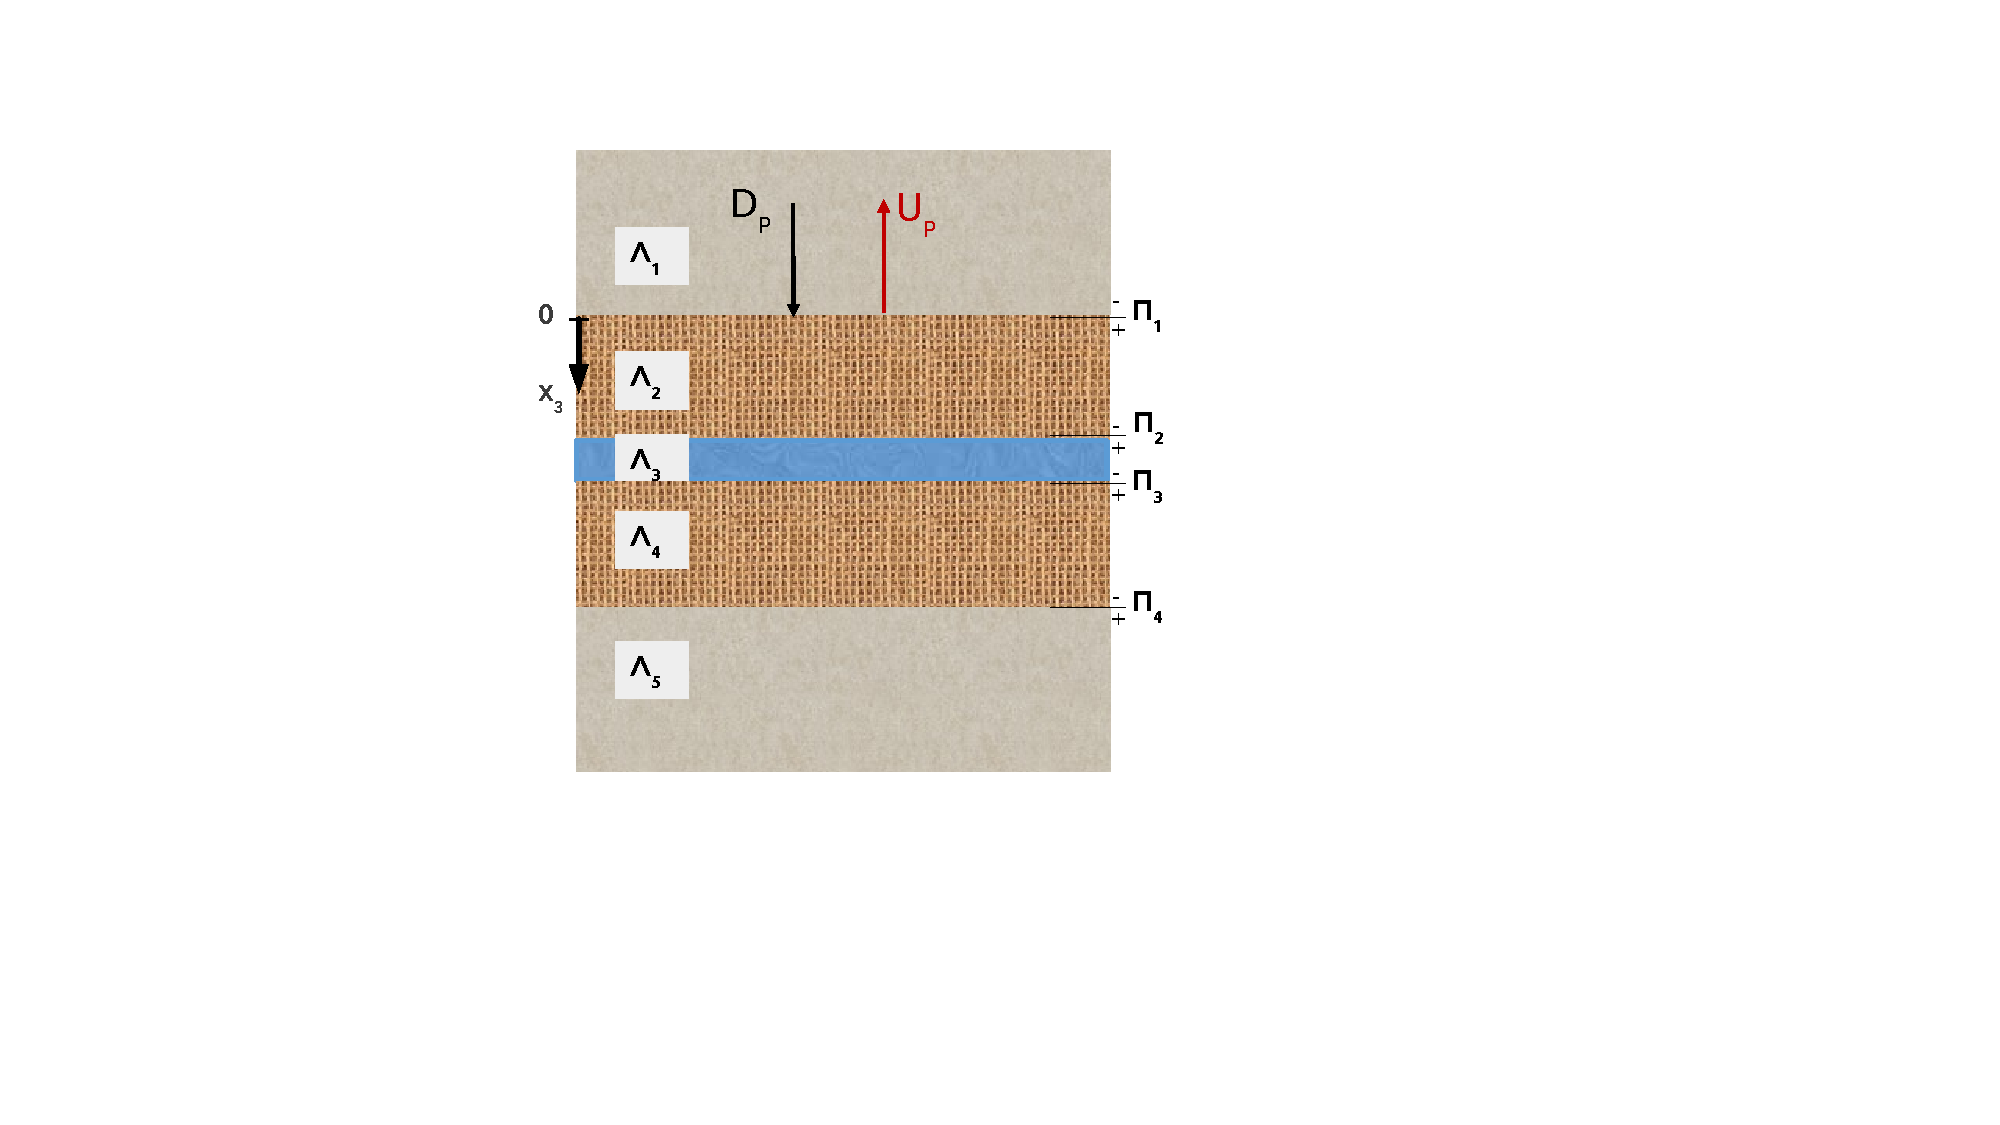
\includegraphics[width= 46mm, height=51mm]{./figures/elastic-poro-model.pdf}
        %\label{}
        }
\subcaptionbox{}{
        \centering
        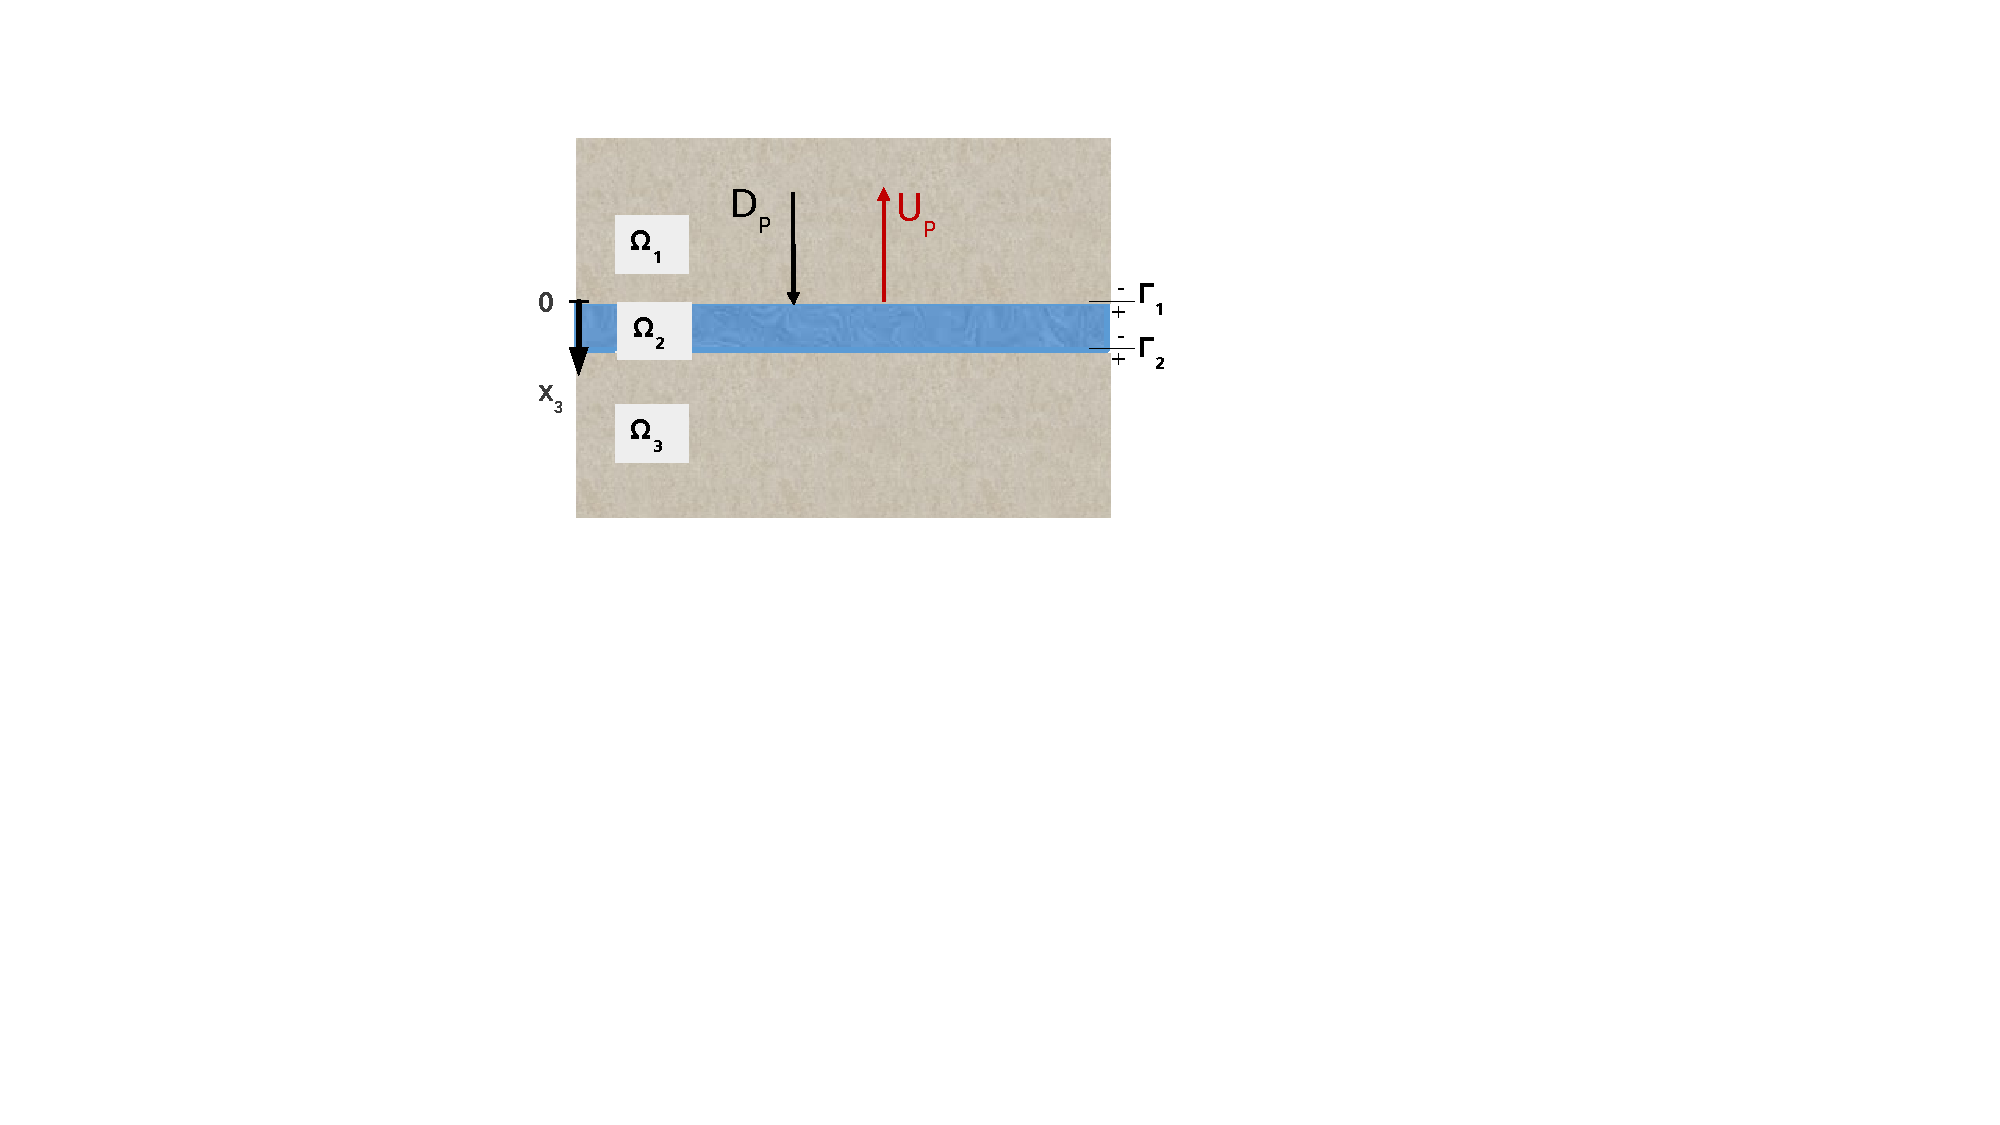
\includegraphics[width=46mm, height=31mm]{./figures/elastic-model.pdf}
        %\label{}
        }
        
\caption{ a) Elastic-poroelastic model. b) Elastic model. $D_P$ and $U_P$ are the incident and reflected P-waves, respectively. }
\label{fig:1}
\end{figure}

We assume a normally incident P-wave striking at the background-DZ interface $\Pi_1$ for the elastic-poro\-elastic model and at the background-fracture interface $\Gamma_1$ for the elastic model. Our objective is to find the corresponding PP reflection coefficients $R_{PP}$. For this, we formulate the poroelastic and elastic wave equations in the space-frequency domain, assuming that the  medium is isotropic. To formulate the poroelastic wave equation,  we let $\mathbf{u}^s =\mathbf{u}^s( \mathbf{x}, \omega)$ and $\mathbf{w} =\mathbf{w}( \mathbf{x}, \omega)$  be the solid displacement vector and the relative fluid displacement vector, respectively, for any position $\bm{x}$ and angular frequency $\omega$. Moreover, we let $\bm{\sigma}$, and $p_f$ be the stress tensor and pore fluid pressure, respectively, which act upon the poroelastic medium. Then, we  express the corresponding equations of motion as \cite{Biot1962}:
\begin{linenomath*}
\begin{equation}\label{Eq.1}
\begin{split}
& -\,\omega^2  \, \rho_b  \, \mathbf{u}^s -  \,\omega^2 \, \rho_f \, \mathbf{w}= \nabla . \, \bm{\sigma}, \\
& -\,\omega^2  \, \rho_f \, \mathbf{u}^s - \omega^2 g(\omega) \, \, \mathbf{w} + i \, \omega \, b(\omega) \, \mathbf{w} = - \nabla \, p_f.
\end{split}
\end{equation}
\end{linenomath*}
The constitutive equations are:
\begin{linenomath*}
\begin{equation}\label{Eq.2}
\begin{split}
& \bm{\sigma} = \mu \,  \left( \nabla \,\mathbf{u}^s + {\nabla  \mathbf{u}^s}^T  \right) + \lambda \, \left( \nabla . \, \mathbf{u}^s\, + \alpha \,M \, \nabla . \, \mathbf{w} \right) \mathbf{I}, \\
&p_f=- \alpha \, M \, \nabla . \, \mathbf{u}^s - M \, \nabla . \, \mathbf{w}, 
 \end{split}
\end{equation}
\end{linenomath*}
where $\rho_b$ and $\rho_f$ are the bulk density of the saturated porous medium and the density of the pore fluid, respectively, $\mu$ is the frame shear modulus, $\phi$ is the porosity of the medium, $I$ is the identity matrix, $i$ is the imaginary unit, $\lambda$ is the undrained Lamé modulus, $\alpha$ is the Biot-Willis effective stress coefficient, $M$ is the Biot's fluid storage modulus, and $g(\omega)$ and $b(\omega)$ are the mass coupling and viscous coefficients, respectively. The required rock physical properties are calculated as follows (e.g., \citeA{Barbosa2016}):

\begin{linenomath*}
\begin{equation}\label{Eq.3}
\begin{split}
& \rho_b =(1-\phi)\rho_s + \phi \rho_f, \\
& \lambda= K_m - \frac{2}{3} \mu + \alpha^2 M, \\
& \alpha =1-\frac{K_m}{K_s},\\
& M  =\left( \frac{\alpha-\phi}{K_s} +\frac{\phi}{K_f} \right)^{-1}, \\
& g(\omega) =  \frac{1}{\omega} \Im \left( \frac{\eta}{\kappa_d(\omega)} \right),\\
& b(\omega) = \Re\left( \frac{\eta}{\kappa_d(\omega)} \right),
\end{split}
\end{equation}
\end{linenomath*}
where $\rho_s$ is the density of the solid grains, $K_m$, $K_s$, and $K_f$ are the bulk moduli of the drained solid frame, the solid grains, and the pore fluid, respectively. Additionally, $\eta$ is the viscosity of the pore fluid and $\kappa_d(\omega)$ is the dynamic permeability of the porous rock, which can be expressed as \cite{Johnson1987}:
\begin{linenomath*}
\begin{equation}\label{Eq.4}
    \kappa_d(\omega)=\kappa \left(\sqrt{1 + \frac{4 i \omega}{n_j \omega_B} }+ \frac{i \omega}{\omega_B}   \right) ^{-1}.
\end{equation}
\end{linenomath*}
%This expression for $\kappa_d(\omega)$ follows the Fourier transform ($\mathcal{F}\{.\}$) convention: $ \mathcal{F} \{\partial f /\partial t \}$ = $i \omega \, \mathcal{F}\{f \}$.
Here, $\kappa$ is the static permeability of the porous medium, $n_j$ is a parameter determined by the pore geometry, and $\omega_B$ is Biot's angular frequency:
\begin{linenomath*}
\begin{equation}\label{Eq.5}
  \omega_B = \frac{\eta \phi}{\rho_f \kappa S},
\end{equation}
\end{linenomath*}
where $S$ is the tortuosity of the pore space. 

To formulate the elastic wave equation, we let $\bm{u}^e=\bm{u}^e (\bm{x},\omega)$ be the displacement vector for any position $\bm{x}$ in the elastic medium and angular frequency $\omega$. We also let $\bm{\sigma}^e$ be the stress tensor field acting upon the medium. Then, we express the corresponding equations of motion as:
\begin{linenomath*}
\begin{equation}\label{Eq.6}
- \, \rho_b \,\omega^2 \, \mathbf{u}^e = \nabla . \, \bm{\sigma}^e.
\end{equation}
\end{linenomath*}
We express the corresponding constitutive equation as: 
\begin{linenomath*}
\begin{equation}\label{Eq.7}
\bm{\sigma}^e = \mu \,  \left( \nabla \, \bm{u}^e + {\nabla  \bm{u}^e}^T  \right) + \lambda \,  \nabla . \, \bm{u}^e\,\, I.
\end{equation}
\end{linenomath*}
 

\subsection{Solution for displacements and PP reflection coefficients}
\subsubsection{Total displacements}
We assume that the incident P-wave propagates downwards, in the $\bm{\hat x_3}$ direction (Figure \ref{fig:1}), where $|\bm{\hat x_3}| =1$, and strikes normally at the interface $\Pi_1$  in the  elastic-poro\-elastic model and at the interface  $\Gamma_1$ in the elastic model. Hence, the only propagating waves in the elastic media are P-waves while in the poro\-elastic layers  are fast P-waves ($P_1$) and slow P-waves ($P_2$). Thus, the only non-zero component of the displacement vectors is in $\bm{\hat x_3}$.
Next, we let
$u{_d^s}$ be the total solid displacement vector component and $w_d$ the total relative fluid displacement vector component, respectively, for the poro\-elastic layer $d$, with $d$ = $\Lambda_2$, $\Lambda_3$ and $\Lambda_4$. Then, we express the component of total displacements as:
\begin{linenomath*}
\begin{equation}\label{Eq.8}
u_d^s =  \sum_q u_{d \,q}^s ,   \qquad
w_d = \sum_q  w_{d \,q}  \;,
\end{equation}
\end{linenomath*}
with $q=D_{P_1},D_{P_2}, U_{P_1},U_{P_2}$, where $D$ and $U$ refer to the downgoing and upgoing waves, respectively, and subscripts $P_1$ and $P_2$ indicate the associated wave mode.
Similarly,  we let $u_n^e$ be the total displacement component for the elastic medium $n$, with $n$ = $\Omega_m$, $\Lambda_1$  and $\Lambda_5$. Here $m = 1,2,3$.  Then, we express  $u_n^e$ as:
\begin{linenomath*}
\begin{equation}\label{Eq.9}
u_n^e = \sum _j u_{n\,j}^e , \; \; 
\end{equation}
\end{linenomath*}
with $j=D_P,U_P$, where subscripts $P$ refers to P-wave. We remark that, for the lower half-spaces $\Omega_3$ and $\Lambda_5$, the displacement is given as ${u_n^e}$ = $u_{n\,D_P}^e $, since there are no upgoing P-waves.

\subsubsection{Solution for displacements}
For the poro\-elastic layers, we express the solution vector component for each solid and relative fluid displacement $u_{d\,q}^s$ and $w_{d\, q}$, as:
\begin{linenomath*}
\begin{equation}\label{Eq.10}
\begin{split}
& u_{d\,q}^s = S_{d\, q}\;\exp[ \pm \; i \; k_{d \,j} \; x_3 ] \, ,\\
& w_{d \,q} = W_{d\,q}\;\exp[\pm \; i\;  k_{d\,j} \;x_3 ] \, ,
\end{split}
\end{equation}
\end{linenomath*}
where $ S_{d\, q}$ and $W_{p\,q}$
are the amplitudes of the corresponding solid and relative fluid displacements, respectively and $x_3$ is the particle position component. Negative and positive signs in the exponential correspond to downgoing and upgoing waves, respectively. Additionally, 
$ k_{d\,j}$ is the poroelastic scalar wave\-number for the wave $j$ in layer $d$, with $j=P_1$ when $q=D_{P_1},U_{P_1}$ and $j=P_2$ when $q=D_{P_2},U_{P_2}$. Pleas note that the scalar wave\-number $ k_{d\,j}$ is complex and frequency-dependent and its real part is associated with the phase velocity. To obtain
$ k_{d\,j}$, we follow the procedure outlined in \citeA{Barbosa2016}.

Similarly, for the elastic media, we express the corresponding solution vector component $u_{n\,j}^e$ as:
\begin{linenomath*}
\begin{equation}\label{Eq.11}
u_{n\,j}^e = E_{n \,j} \;\exp[ \pm\; i \; k_{n}^e \; x_3 ]\,,
\end{equation}
\end{linenomath*}
where $E_{n \,j}$ is the amplitude of the corresponding elastic displacement and $ k_{n}^e$ is the elastic scalar wave\-number for the P-wave in medium $n$, calculated as $ k_{n}^e$ = $\omega / V_P^n$, where $V_P^n$ is the P-wave velocity of medium $n$. 
%We also assume that the elastic layer $n$ exhibits an undrained behavior.
Following \citeA{Gassmann1951}, the corresponding $V_P^n$ can then be expressed as:
\begin{linenomath*}
\begin{equation}\label{Eq.12}
V_P^n = \sqrt{\frac{\lambda^n +  2\, \mu^n}{\rho_b^n}} .
\end{equation}
\end{linenomath*}
Here, $\lambda$ and $\rho_b$ are the undrained Lamé modulus and the bulk density as defined in equation (\ref{Eq.3}).

\subsubsection{PP Reflection coefficient}
We aim to find the PP reflection coefficients $R_{PP} = \tensor*[]{E}{_n_{\, \text{\tiny $U_P$}}}/ \tensor[]{E}{_n_{\, \text{\tiny $D_P$}}}$, where  $n$ refers to either the upper half-space $ \Lambda_1$ in the elastic-poro\-elastic model (Figure \ref{fig:1}a) or the upper half-space $\Omega_1$ in the elastic model  (Figure \ref{fig:1}b).
Moreover, without loss of generality, we assume that $ \tensor[]{E}{_n_{\, \text{\tiny $D_P$}}}$ = $1$. Then, we seek to find ${E}_{n\, \text{\tiny $U_P$}}$ together with the other amplitudes of the displacements in the  media $\Lambda_q$ of the elastic-poroelastic model (Figure \ref{fig:1}a), with $q=1,..,5$ and  in the media $\Omega_q$ of the elastic model (Figure \ref{fig:1}b), with $q=1,2,3$. To this end,
we assemble sets of linear equations, which we find by imposing the continuity of different physical quantities at the corresponding media interfaces.

For the elastic-poroelastic model, we distinguish two types of interfaces: elastic-poroelastic and purely poroelastic ones. At the elastic-poroelastic interfaces $\Pi_q$, for  $q=1,4$,
we impose the continuity of solid displacements and tractions and we set to zero the relative fluid displacements, respectively \cite{Deresiewicz1963}: 
\begin{linenomath*}
\begin{equation}\label{Eq.13}
\begin{split}
&  \left. \left(  u_n^e -  u_d^s \right) \right \rvert_{\Pi_q} = 0 \,, \\
&  \left. \left(  t_n^e -  t_d \right) \right \rvert_{\Pi_q} = 0 \,,\\
& \left.  w_d^s \right \rvert_{\Pi_q} = 0 \,.
\end{split}
\end{equation}
\end{linenomath*}
For $q=1$, the corresponding media are $n=\Lambda_1$ and $d=\Lambda_2$, for $q=4$, they are $n=\Lambda_5$ and $d=\Lambda_4$.
We calculate the traction component $t_n^e$ as $t_n^e$ = $ ({\bm{\sigma}^e} \,^{\bm{.}} \,\bm{\hat x_3}) \, ^{\bm{.}} \, \bm{\hat x_3}$. Then, using equation (\ref{Eq.7}) to replace $\bm{\sigma}^e$, we express $t_n^e$ as:
\begin{linenomath*}
\begin{equation}\label{Eq.14}
t_n^e =(\lambda^n + 2 \mu^n)\,  \left( \, u_n^{e} \, \right)_{,3} \,,
\end{equation}
\end{linenomath*}
where  $(^.)_{,3}$ = $\partial (^.)/ \partial{x_3}$. 

Similarly,  we calculate the traction component $t_d$ as $t_d$ = $(\bm{\sigma} \, ^{\bm{.}} \, \bm{\hat x_3}) ^{\bm{.}} \, \bm{\hat x_3}$ and, using equation (\ref{Eq.2}) to replace  $\bm{\sigma}$, we express $t_d$ as:

\begin{linenomath*}
\begin{equation}\label{Eq.15}
t_d =  (\lambda^d + 2 \mu^d)\,  \left( \, u_d ^s \, \right)_{,3}\; + \alpha^d M^d \,  \left( \, w_d \right)_{,3} \,.
\end{equation}
\end{linenomath*}

At the purely poroelastic interfaces $\Pi_q$ with $q=2,3$, we impose the continuity of solid displacements, relative fluid displacements, tractions and pressures, respectively \cite{Deresiewicz1963}:
\begin{linenomath*}
\begin{equation}\label{Eq.16}
\begin{split}
&  \left. \left( u_d^s -  u_{(d+1)}^s \right) \right \rvert_{\Pi_q} = 0 \,, \\
&  \left. \left(  w_d -  w_{(d+1)} \right) \right \rvert_{\Pi_q} = 0 \,, \\
& \left . \left(  t_d  - t_{(d+1)}  \right) \right \rvert_{\Pi_q}= 0 \,,\\
&  \left. \left(  p_{f\,d} -  p_{f\, (d+1)} \right) \right \rvert_{\Pi_q} = 0 \,.
\end{split}
\end{equation}
\end{linenomath*}
Here, $d$ =$\Lambda_q$ and ($d+1$) = $\Lambda_{(q+1)}$. Moreover, we calculate $t_d$ and $t_{(d+1)}$ using equation (\ref{Eq.15}). 
Additionally, using equation (\ref{Eq.2}), we evaluate the pore pressure:
\begin{linenomath*}
\begin{equation}\label{Eq.17}
p_{f \, d} = - \alpha^d M^d\,  \left( \, u_d^{s} \, \right)_{,3}\; - M^d \,  \left( \, w_d \right)_{,3} \, .
\end{equation}
\end{linenomath*}
To complete the system of equations, we express the relative fluid displacement in terms of the solid displacement through
 $\tensor []{\gamma}{_d_{\,j}}=\tensor*[]{W}{_d_{\, j}}/\tensor*[]{S}{_d_{\, j}}$ where $j=P_1, P_2$. This ratio can be  obtained from the properties of the porous medium \cite{Barbosa2016}.
 
For the elastic model, we obtain the corresponding system of equations by imposing the continuity of displacements and tractions  at each medium interface $\Gamma_q$ with $q=1,2$, respectively:
\begin{linenomath*}
\begin{equation}\label{Eq.18}
\begin{split}
&  \left. \left(  u_n^e -  u_{(n+1)}^e \right) \right \rvert_{\Gamma_q} = 0 \,, \\
&  \left. \left( t_n^e  - t_{(n+1)}^e  \right) \right \rvert_{\Gamma_q} = 0 \,.
\end{split}
\end{equation}
\end{linenomath*}
Here $n$ = $\Omega_q$ and ($n+1$) = $\Omega_{(q+1)}$. We calculate $t_n^e$  and $t_{(n+1)}^e$ using equation (\ref{Eq.14}).

% This is the ratio of the reflected P wave amplitude ($ \tensor[]{E}{_n_{\, \text{\tiny $U_P$}}}$) to the incident P wave amplitude 
% (\,$ \tensor[]{E}{_n_{\, \text{\tiny $D_P$}}}$) at the upper half space boundary $\tensor*[]{\Gamma}{_1^+}$ or $\tensor*[]{\Pi}{_1^+}$. 
 
 We have set up the solution for displacements  in such a way that the reflection coefficient for the elastic-poroelastic model matches that of the elastic model at the high frequency limit. This is the result of considering plane wave displacements and of assigning the same rock properties for the DZ and the background. Under this consideration, in the high frequency limit the DZ presents the same seismic response as the background and, therefore, it  makes no difference calculating the reflection coefficient at the DZ-fracture interface or at the background-fracture interface.

\subsection{FPD frequency regimes}
%FPD occurs in porous background rocks that present inclusions exhi\-biting contrasting elastic properties.
When seismic waves propagate through heterogeneous materials, pore fluid pressure perturbations arise between regions of differing compresibilities. These pressure gradients are equilibrated through FPD, which, depending on the underlying heterogeneities, prevails at different scales. Our analysis focuses in the mesoscopic scale, which refers to those heterogeneities that are larger than the pore size but much smaller than the wavelength of the propagating wave. For the case of compliant fractures embedded in a much stiffer DZ, the compressi\-bility contrast allows seismic waves to induce strong fluid pressure gradients and  associated fluid flow.

On the other hand, it is important to notice that FPD prevails at frequencies much lower than Biot's characteristic frequency: $f$ $\ll$ $f_B$, with $f_B$ =$\omega_B/(2 \pi)$ (equation \ref{Eq.5}). At these sufficiently low frequencies, the fluid flow within the pores is viscous-dominated,  provided that the thickness of the viscous boundary layer remains greater than the characteristic pore size \cite{Johnson1987}. Under this condition, the  imaginary part of the dynamic permeability $k_d (\omega)$ becomes negligible (equation \ref{Eq.4}).
Moreover, in the low frequency limit, $k_d (\omega)$  becomes real-valued and frequ\-ency\--independent and equal to the static permeability $\kappa$: $ \lim \limits_{\omega \to 0}k_d (\omega)$ = $\kappa$. If we additionally constrain the analysis of Biot's equations to the quasi-static case, it can be shown that the behavior of the slow P-wave is described by a pressure diffusion equation with diffusion coefficient $D$ \cite{Chandler1981}: 
\begin{linenomath*}
\begin{equation}\label{Eq.19}
D = \frac{\kappa}{\eta} \frac{M H_d}{H},
\end{equation}
\end{linenomath*}
where the drained and undrained plane-wave moduli $H_d$ and $H$ can be calculated as $H_d= K_m + 4/3 \,\mu$ and $H = \lambda + 2 \mu$, respectively. Moreover, we let  $L_d$ be the characteristic diffusion length which can be expressed as \cite{Norris1993}: 
\begin{linenomath*}
\begin{equation}\label{Eq.20}
L_d = \sqrt{\frac{D}{\omega}}.
\end{equation}
\end{linenomath*}
As frequency varies, distinct FPD regimes can be identified according to the relative magnitudes between the scale of a heterogeneity and its characteristic diffusion length. For the case of a fracture embedded in a DZ, the relevant scales are their respective thicknesses. For simplicity, let us assume that the thickness of the fracture $h^c$ is negligible compared to that of the DZ and that its permeability is so high that for practical terms it does not pose any restriction for fluid flow. In this context, we have $h^c \ll L_d^c$ for the frequency range of interest. Here, the superscript $c$ refers to the fracture. Conversely, if we consider that the DZ thickness is much larger than that of the fracture but its permeability is much lower, then we expect that the relationship between DZ thickness $h^z$ and its characteristic diffusion length $L_d^z$  varies from $h^z\ll L_d^z$  to $h^z\gg L_d^z$ as frequency increases.
Thus, for the fracture-DZ poroelastic system, we can regard the thickness of the DZ $h^z$ as the relevant mesoscopic heterogeneity scale controlling FPD. Under this perspective, we  distinguish the following two end-member regimes for FPD: relaxed and unrelaxed. The relaxed state occurs at sufficiently low  frequencies, at which the diffusion length $L_d^z$ is larger than the thickness of the DZ $h^z$.
Thus, there is enough time for the pressure between the fracture and DZ layers to equilibrate. Conversely, the unrelaxed state occurs at sufficiently high frequencies, at which the diffusion length $L_d^z$ is very small compared to thickness of the DZ $h^z$ and, consequently, there is no time for FPD to take place, and the medium behaves as hydraullically isolated. A transition zone exists at intermediate frequencies, at which the diffusion lengths are of comparable size to that of the thickness of the DZ $h^z$. This zone is characterized by a transition frequency $f_c = \omega_c /2 \pi$, which can be estimated as \cite{Brajanovski2006, Muller2006}: 
\begin{linenomath*}
\begin{equation}\label{Eq.21}
   w_c \approx  \frac{9}{2} \frac{D^z}{(h^z)^2}  ,
\end{equation}
\end{linenomath*}

In this work, we consider an open fracture whose permeability is several orders of magnitude greater than the DZ. Then, it is possible that $f_B^c$ $<<$ $f_B^z$, meaning that FPD within the fracture is limited to much lower frequencies than within the DZ. Particularly, for frequencies greater than $f_B^c$ but lower than $f_B^z$, FPD does no longer take place within the fracture since fluid flow becomes inertial-dominated, but FPD is still present within the DZ.  We remark that, the proposed solutions for amplitude displacements, as expressed in equation (\ref{Eq.10}), account for both fluid flow regimes viscous- and inertial-dominated since they include the dynamic permeability (equation \ref{Eq.4}) in the calculation of the poroelastic wavenumbers  of the fracture and DZ. Therefore,
within this frequency band, pressure equilibration will take place under two different flow regimes. Nonetheless, due to the greater thickness and lower permeability of the DZ, it is expected that the viscous-dominated fluid flow regime in this region controls the response of the DZ-fracture system.
% at the fracture-DZ boundary, the propagating $P_2$ at the fracture side converts to a diffusive $P_2$ at the DZ side. The resonant effects of the propagating $P_2$ within the fracture are likely to be seen in frequencies higher than seismic exploration band due to the vanishing small thickness of the fracture.



\subsection{Normal fracture compliance}
% \cite{schoenberg1980elastic}, in an elastic context, defines fracture compliance 
% as the parameter relating the displacement jump and traction across a discontinuity idealized as a slip interface.
Fracture compliance defines the mechanical behavior of a fracture. The more compliant a fracture is, the easier it undergoes deformation and the higher is its reflectivity since the mechanical contrast with the background increases. For the case of FPD effects caused by a normally incident P-wave, our interest focuses on normal fracture compliance. For the fracture-DZ poroelastic system, FPD  allows fluid flow from the more compliant fracture to the stiffer DZ during half of a wave cycle, which, in turn, decreases the stiffening effect of the fracture fluid, thus 
increasing the normal compliance of the fracture and its reflectivity.
% Thus, for the fracture-DZ poroelastic system, softening effects on the fracture compliance as a consequence of FPD between such regions increases reflectivity.
However, the extent to which normal fracture compliance and its reflectivity increase
is controlled by the FPD regimes. Normal compliance is maximal,  with maximal increase of reflectivity, when FPD is in its relaxed state, that is, when the fracture fluid is allowed to exit until the pressure fully equilibrates. In contrast,  normal fracture compliance is lowest with no reflectivity enhancement during the unrelaxed FPD regime, in which the fracture behaves as hydraulically isolated. Intermediate values of normal fracture compliance are expected as FPD transitions from its relaxed to its unrelaxed regime.

We calculate the normal fracture compliance  $Z_N^e$ for the elastic thin layer model using the definition introduced by \citeA{schoenberg1980elastic}. Then, extending this concept to a poroelastic framework in a similar way to \citeA{Rubino2015a}, we calculate the normal fracture compliance $Z_N^p$ for the poroelastic thin layer model:
\begin{linenomath*}
\begin{equation}\label{Eq.22}
\begin{split}
& Z_N^e =  \frac{ \left.u_{n}^e \right \rvert_{\Gamma_2} - \left.u_{n}^e \right \rvert_{\Gamma_1}}{\bar t^{\,e}_n},  \quad \text{with} \quad
\bar t^{e}_{n} = \frac{ \left.t^{e}_{n} \right \rvert_{\Gamma_1}+ \left.t^{e}_n \right \rvert_{\Gamma_2}}{2}\; , \\
& Z_N^p =  \frac{ \left.u_{d }^s \right \rvert_{\Pi_3} - \left.u_{d}^s \right \rvert_{\Pi_2}}{\bar t_d},  \quad \text{with} \quad
\bar t_{d} = \frac{ \left.t_{d} \right \rvert_{\Pi_2}+ \left.t_{d} \right \rvert_{\Pi_3}}{2} \;.
\end{split}
\end{equation} 
\end{linenomath*}
Here, $n$ = $\Omega_2$, $d$ = $\Lambda_3$.

% For comparison, we also calculate the poroelastic normal fracture compliance by applying the poroelastic linear slip (PLS) theory proposed by \citeA{Nakagawa2007}. They express the jump in solid displacement $\Delta u^s$ across an open fracture interface as: $\Delta u^s = Z_n^d (\sigma_{\text{\tiny (33)}} + \alpha \, p_f)$. Here, $Z_N^d$ is the drained normal fracture compliance which is defined as: $Z_N^d$ = $h^c/H_d^c$,
% Then, to obtain the poroelastic normal compliance ($Z_N^{PLS}$), we divide the jump in displacement $\Delta u^s$ by the total traction:
% \begin{linenomath*}
% \begin{equation} \label{Eq.23}
% Z_N^{PLS} = Z_N^d \; \frac{\bar t^{d}_{ \text{\tiny (3)}} }{ \bar t_{ \text{\tiny (3)}}  }  \quad \text{with} \quad
% \bar t^{d}_{\text{\tiny (3)}} = \frac{  t^{d}_{\text{\tiny (3)}} \rvert_{\Pi_2} +  t^{d}_{\text{\tiny (3)}}  \rvert_{\Pi_3}}{2},
% % & Z_N^{P_1}=   \frac{ \left.u^s_{P_1} \right \rvert_{\Pi_3^+} -  \left.u^s_{P_1} \right \rvert_{\Pi_2^-}  }{\bar t^{\,p}_{P_1\text{\tiny (3)} } } \quad \text{with} \quad
% % \bar t ^{\,p}_{P_1 \text{\tiny (3)} }= \frac{ t^p_{P_1 \text{\tiny(3)} } \rvert_{\Pi_2^-} + t^p_{P_1 \text{\tiny(3)} }  \rvert_{\Pi_3^+} }{2},\\[5pt]
% % &Z_N^{LS}= \frac{2 \,R_{PP}}{  (\rho_b^n V_P^n ) (1+R_{PP}) i \omega }
% \end{equation}
% \end{linenomath*}
% where $ t^{d}_{\text {\tiny (3)}} $= $\sigma_{\text{\tiny (33)}} + \alpha p_f$.

% Moreover $ t^{d}_{\text {\tiny (3)}} $ can be interpreted  as the traction component normal to the fracture plane  acting upon the frame of the porous rock.
% $\tensor*[]{Z}{_N^{\text{\tiny $P_1$}}}$ is calculated only with $P_1$ displacements as in \citeA{Barbosa2017} and 
% $\tensor*[]{Z}{_N^{\text{\tiny LS}}}$ is estimated applying the elastic linear slip (LS) theory \cite[]{schoenberg1980elastic} for the reflection of a normal incident P-wave at an slip interface. For this estimation, we use the reflection coefficient $R_{PP}$ resulting from the elastic-poroelastic model analysis. In this equation, the superscript $n$ refers to the elastic half-space.

On the other hand, following \citeA{Rubino2015a}, we express the low- and high-frequency limits of normal fracture compliance, $Z_N^o$ and $Z_N^u$ as:
\begin{linenomath*}
\begin{equation} \label{Eq.23}
\begin{split}
 & Z_N^o= Z_N^u + \frac{2 B^{c} \left(B^c-B^z \right)}{ \frac{2 B^c}{\alpha^z Z_N^d} + \frac{M^z(1-\alpha^z B^{z})}{h^z} }\,,\\
 & Z_N^u= \frac{h^{c}}{H^{c}}\,.
\end{split}
\end{equation}
\end{linenomath*}
%= $\sigma^{pd}_{\text{\tiny 33}} \rvert_{\Pi_q}$ 
Here $B$ is the Skempton coefficient, which can be expressed as $B=\alpha M/H$.  $Z_N^o$ and $Z_N^u$ are the maximum and minimum values that the normal compliance of a fracture can take for a given set of rock and fluid properties. These limiting values correspond to the relaxed and unrelaxed FPD regimes, respectively. In particular, the high-frequency limit of fracture normal compliance $Z_N^u$ correspond
to the elastic behavior of the fracture and, as detailed by equation (\ref{Eq.23}), its value only depends on the fracture physical properties. In this work, we use the ratio $Z_N^o/Z_N^u$ as a measure of the maximum increase of normal fracture compliance due to FPD with respect to its elastic limit value.
\citeA{Rubino2015a} find the expressions for $Z_N^o$ and $Z_N^u$ by considering a one-dimensional periodic system consisting of a relatively thick horizontal layer alternating with a thinner layer representing a fracture. They assume a representative elementary volume (REV) comprised of the fracture layer and the two thicker embedding layers with half of their thickness. 
They also assume a no flow condition at the  upper and lower boundaries of the REV, which holds for the entire system given the symmetry of the problem and its infinite nature. For  the fracture-DZ poroelastic system enclosed within elastic half-spaces considered in this work, periodicity is no longer required to ensure the no flow condition since this is in fact imposed by the zero relative fluid displacement boundary condition at the the interfaces between the poroelastic DZ and elastic half-spaces representing the impermeable background (equation \ref{Eq.13}). Thus, the expressions in equation (\ref{Eq.23}) are applicable for our problem when we consider the entire thickness of the DZ.
%*****************
%RESULTS
%*****************
\section{Results}
In  the following examples, we present results of frequency-dependent reflectivity and normal fracture compliance for different values of DZ permeability. First, we show results using rock and fluid properties from Table \ref{fig:1}. These results are used as a reference for comparison with the examples that follow. The next examples show also frequency-dependent reflectivity and normal fracture compliance, but with different rock and fluid  properties which we vary at a time except for the fluid properties. For the DZ, we change its thickness, porosity and moduli. For the fracture, we change its moduli and for the fluid, we change its bulk modulus and viscosity. For these examples, we  use the same rock properties for the DZ and the background to allow the match of reflectivities at high frequencies between the elastic-poroelastic and the elastic models.

Table \ref{table:1} shows the reference values of the rock and fluid properties for the poroelastic thin layer representing the fracture and the associated DZ layers. Most of these values are adopted from  \citeA{Barbosa2016} and \citeA{Barbosa2019}, with rock properties emulating that of a crystalline lithology. Fracture bulk and shear moduli, $K_{m}^c$ and $\mu^c$, are estimated using the formulae proposed by \citeA{Nakagawa2007}:
\begin{linenomath*}
\begin{equation} \label{Eq.24}
Z_T^d=h^c/\mu^c ; \qquad Z_N^d=h^c/(K_{m}^c + 4/3 \, \mu^c).
\end{equation}
\end{linenomath*}
For the drained tangential $Z_T^d$ and normal $Z_N^d$ compliances, we assume values of  \num{5e-10} m/Pa and \num{1.5e-10} m/Pa, respectively. The order of these values ($\num {e-10}$) is suggested to correspond to a fracture of around a hundred meters \cite{Hobday2012}.
For the elastic media, comprised by the elastic fracture and half-spaces, we compute the corresponding elastic moduli using Gassmann's equations \cite{Gassmann1951} and taking the required rock and fluid properties from Table \ref{table:1}. For calculations corresponding to the half spaces, we take the necessary rock properties from the ones listed for the DZ and, in a similar way, for the elastic fracture we take the required properties from the poroelastic fracture. We indicate that, for the rock and fluid properties listed in Table \ref{table:1}, the Biot's frequency for the DZ and fracture is \num{8.1e3} Hz and \num{1.2e3} Hz, respectively.
%Then, the respective drained plane-wave modulus $H_d^c$ is 6.7e-3 GPa.

\begin{table}[!ht]
  \caption{Reference values of the physical properties for the DZ, fracture and pore fluid.}
\begin{center}
  \begin{tabular}{ | l | c | c| }
    \hline
    Property & DZ & Fracture \\ \hline
    Grain bulk modulus $K_s$ ($GPa$) & 37 & 37 \\ 
    Grain density $\rho_s$ ($Kg/m^3$) & 2730 & 2730 \\
    Porosity $\phi$ & 0.015 & 0.8 \\
    Frame bulk modulus $K_m$ ($GPa$) & 33 & 0.004\\ 
    Frame shear modulus $\mu$ ($GPa$) & 29 & 0.002 \\
    Thickness $h$ ($m$) & 0.2 & 0.001\\ 
    Permeability $\kappa$ ($D$) & 0.1 & 100\\
    Tortuosity $S$ & 3 & 8\\
    Fluid density $\rho_f$ ($Kg/m^3$) & 1000 & 1000\\
    Fluid bulk modulus $K_f$ ($GPa$) & 2.25 & 2.25\\
    Fluid viscosity $\eta$ ($Pa.s$)& 0.001 & 0.001\\
    Pore geometry parameter $n_j$ & 8 & 8\\
    \hline
  \end{tabular}
  \label{table:1}
\end{center}
\end{table}


Next, we  present plots of reflectivity (Figure \ref{fig:2}) and of the corresponding  normal fracture compliance  (Figure \ref{fig:3}) using the rock and fluid properties of Table \ref{table:1}.
% We also remark that this and the following examples show that the presence of the DZ enhances the fracture normal compliance and, as a consequence, its reflectivity in the seismic frequency range compared to a hydraulically isolated fracture. This is the consequence of the existence of a permeable DZ that allows fluid exchange with the main fracture.
Specifically, Figure \ref{fig:2} shows the absolute value of the reflection coefficient $|R_{PP}|$ versus frequency for the elastic and the elastic-poroelastic models considering different DZ permeabilities $\kappa^z$. These results show that there is a maximum increase of reflectivity for the elastic-poroelastic models of approximately one-order-of magnitude when compared to the elastic results for frequencies less than the respective transition frequencies $f_c$. This is a consequence of FPD prevailing between the DZ and the fracture, which allows fluid release from the fracture as the pressure equalizes during a half wave cycle. 
% This, in turn, increases normal fracture compliance (Figure  \ref{fig:5}) and, consequently, also the reflectively of the system.
Furtheremore, this increase is controlled by the thickness $h^z$ 
%and the permeability $\kappa^z$
of the DZ. We observe that, for the given DZ thickness, $h^z$ = 0.2 m, there is an upper limit for $|R_{PP}|$ regardless of the permeability $\kappa^z$. This happens because the DZ thickness provides a limited pore volume for FPD to occur in its relaxed state. Moreover, the permeability $\kappa^z$ controls the transition frequency at which reflectivity decreases towards its undrained values and  higher permeabilities shift this transition frequency towards higher values. This is expected given that the characteristic transition frequency $f_c$ is directly proportional to the permeability $\kappa^z$ (equations \ref{Eq.19} and \ref{Eq.21}). We also observe the presence of reverberations at high frequencies for the $|R_{PP}|$ curve corresponding to a permeability of 1 D. In this respect, we remark that the corresponding Biot's frequency in the DZ is $ \sim$ 800 Hz and that at this frequency $P_2$ becomes a propagating wave. Then, multiples are expected within the DZ layer when the wavelength of $P_2$ becomes at least two times smaller than the layer thickness. Furthermore, at frequencies comparable to or larger than Biot's frequency, the relaxation mechanism is no longer controlled  by viscous diffusion but by inertial forces. In that case, equations (\ref{Eq.19}) to (\ref{Eq.21}), which assume a pressure diffusion mechanism, no longer apply.

\begin{figure}
\centering

        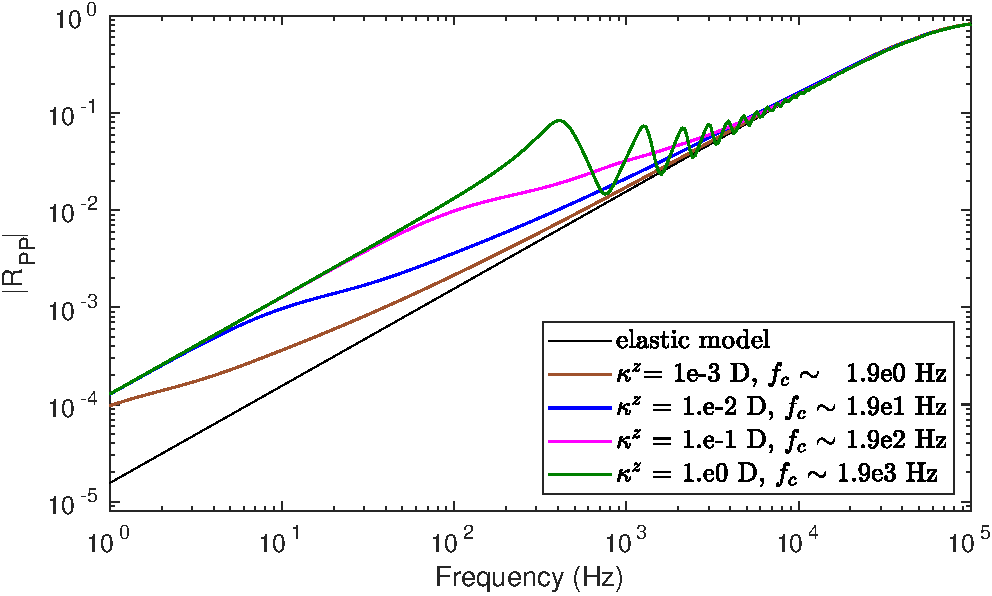
\includegraphics[width=80mm, height=50mm]{figures/elasporo_1mm_ksen_h20e-2.pdf}
        %\label{}
        
    % \subcaptionbox{}
    %   {0
    %     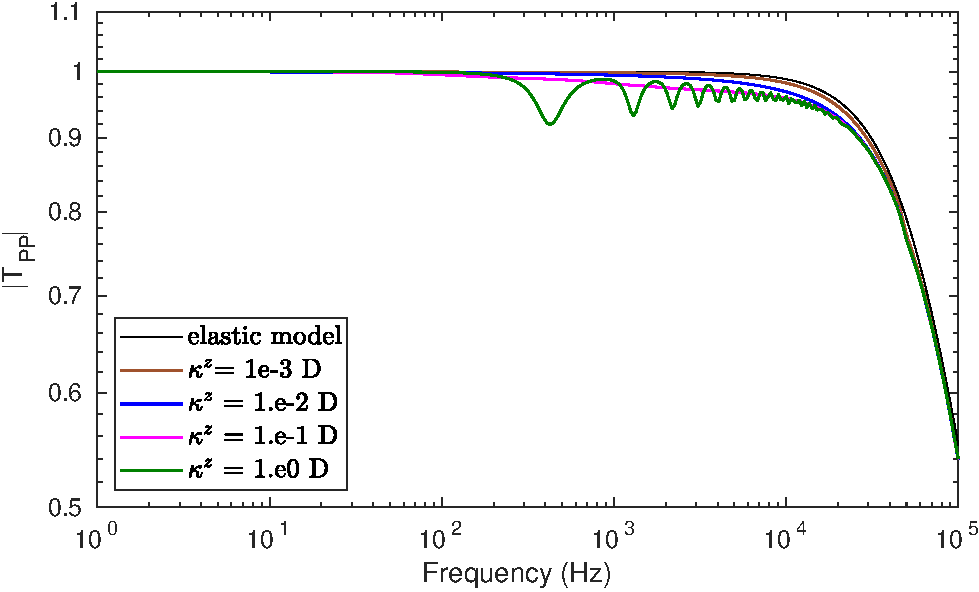
\includegraphics[width=80mm, height=50mm]{figures/TPPelasporo_1mm_ksen_h20e-2.pdf}
    %     %\label{}
    %     }
\caption {Absolute value of normal P-wave reflectivity $|R_{PP}|$ as a function of frequency for different DZ permeabilities $\kappa^z$.}
% (b)  Absolute value of normal P-wave transmission coefficient  $|T_{PP}|$ as a function of frequency for different DZ permeabilities $\kappa^z$.
\label{fig:2}
\end{figure}

Figures \ref{fig:3}a and \ref{fig:3}b show the real and imaginary parts of the normal fracture compliance, respectively, as a function of frequency for different values of the DZ permeability 
$\kappa^z$. We use equation (\ref{Eq.22}) to calculate both the elastic normal fracture compliance $Z_N^e$ and the poroelastic normal fracture compliance $Z_N^p$, respectively. As expected, the elastic normal compliance $Z_N^e$ is constant for all frequencies and presents the lowest compliance value, thus, indicating the undrained limit. In contrast, the poroelastic normal compliance $Z_N^p$  becomes complex-valued and frequency-dependent as the FPD regime transitions from the relaxed  to the unrelaxed states.  $Z_N^p$ reaches its lowest value at the high-frequency limit, 
at which matches the elastic fracture compliance.
% Thus, FPD induced by the presence of DZ can explain the existence of complex-valued fracture compliance in impermeable rocks as.
We point out that experimental support for the frequency-dependence of normal fracture compliance in poroelastic media has been provided by the work of \citeA{Nakagawa2013}. This study presents results of fracture stiffness (inverse of compliance) as a function of frequency for a fluid saturated fracture, showing curves with similar trends as those in Figure \ref{fig:3}a.
Regarding the behavior of normal fracture compliance at the low-frequency limit, Figure \ref{fig:3}a shows that,
at sufficiently low frequencies, the values of $Re[Z_N^p]$ are highest since the fracture experiences the maximum deformation while the maximum fluid exchange occurs between the DZ and the fracture. Nonetheless, there is an upper limit for $Re[Z_N^p]$ regardless of the DZ permeability, which is constrained by the DZ thickness $h^z$. This is because $h^z$ limits the pore volume available for FPD. 
In addition, using equation (\ref{Eq.23}), we obtain the fracture normal compliance for thethe low-frequency limit, $Z_N^o$ = \num{3.4e-12} m/Pa and the
high-frequency limit, $Z_N^u$ =  \num{3.6e-13}  m/Pa, respectively, which corresponds to a ratio $Z_N^o/Z_N^u$ equal to 9.45. To corroborate the accuracy of these results, we also estimate the average normal compliance for these frequency limits directly from the plots presented in Figure \ref{fig:3}a. To this end, we use the results from the curves with $k^z$ equal to \num{e-2} D and \num{e-1} D at a frequency of 1 Hz for the low-frequency limit and at a frequency of \num{4.5e4} Hz for the high-frequency. This yields \num{3.39e-12} m/Pa and \num{3.65e-13} m/Pa for the average compliances in the low- and high-frequency limits, respectively. Comparing these results with the ones obtained using equation (\ref{Eq.23}), we find that the errors are of the order of 1 \% or less.
Moreover, as remarked for Figure \ref{fig:2}, the DZ permeability controls the transition frequency towards the undrained normal compliance. The estimated values  for the respective transition frequencies are presented in Figure \ref{fig:2}. Overall, these results indicate that FPD effects increase the normal fracture compliance as fluid exchange occurs between the fracture and the DZ, which, in turn, increases the reflectivity of the system. Our results also suggest that a possible explanation for the existence of an imaginary part in seismic measurements of  normal fracture compliance is the presence of FPD effects between the fracture and associated DZ even if the background is largely impermeable  \cite{Barbosa2019}.


\begin{figure}
\centering
    \subcaptionbox{}
      {
       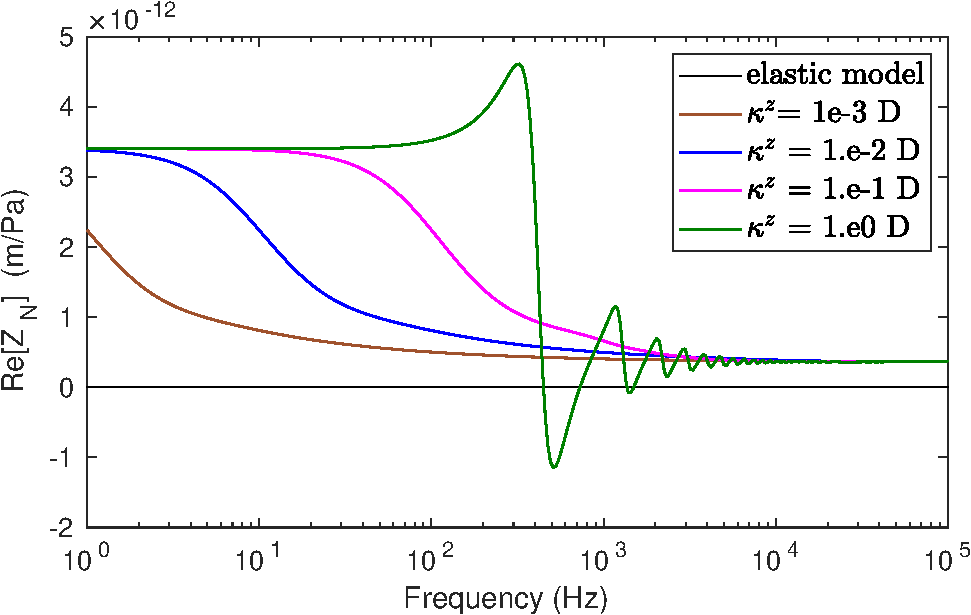
\includegraphics[width=73mm, height=43 mm]{figures/elasporo_1mm_znsen_h20e-2.pdf}
        %\label{}
        }
    \subcaptionbox{}
      {
        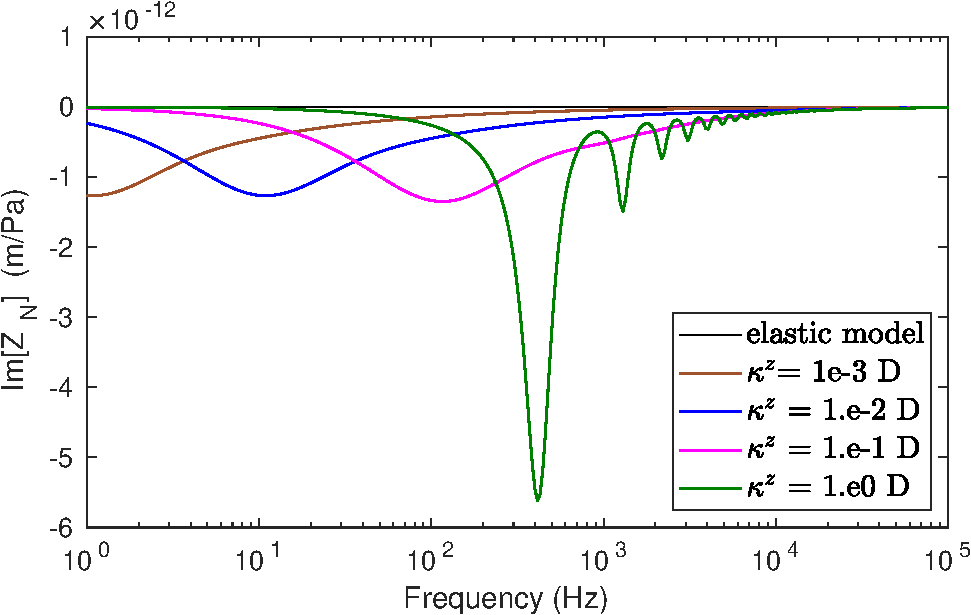
\includegraphics[width=73mm, height=43mm]{figures/elasporo_1mm_iznsen_h20e-2.pdf}
        %\label{}
        }
\caption {(a) Real and (b) imaginary parts of  normal fracture compliance $Z_N$ as a function of frequency for different DZ permeabilities $\kappa^z$. } 
\label{fig:3}
\end{figure}

\subsection{Effect of thickness and porosity of the DZ}
The thickness and porosity of the DZ determines the pore volume available for fluid flow  due to FPD into the DZ. Thus, in the following examples (Figures \ref{fig:4} and \ref{fig:5}) we show that as the thickness and porosity of the DZ increase, so do FPD  and, therefore, the maximum normal fracture compliance and reflectivity of the system. 

Correlations from field data suggest that the thickness of  DZ  measured from the fault core can vary from centimeters to kilometers and is likely to scale with fault displacement  \cite{Mitchell2009, Faulkner2011}. In contrast, field measurements and estimations of DZ surrounding magma driven veins are in the order of centimeters and meters \cite{Engvik2005}. 
For this example (Figure \ref{fig:4}), we consider the effect on reflectivity and normal fracture compliance of variations of the DZ thickness  from five centimeters to close to one meter (0.8 m). These thicknesses would  correspond to fault displacements of less than some tens of a meter  \cite{Mitchell2009, Faulkner2011} and to fault lengths of less than one kilometer \cite{Cowie1992}.
In particular,
Figure \ref{fig:4}a shows $|R_{PP}|$ as a function of frequency for a DZ permeability $ \kappa^z $ of 0.1 D and varying values of DZ thickness $h^z$. Figure \ref{fig:4}b shows the real part of $Z_N$ for the same DZ parameters. We notice that both the maximum value of $|R_{PP}|$ and $Z_N$ increases with increasing thickness $h^z$. This occurs because a wider DZ thickness provides more pore volume for FPD to happen in its relaxed regime, and as a consequence more fluid is allowed to exit the fracture increasing its normal compliance and the reflectivity of the system.
On the other hand, an increase in DZ thickness shifts the characteristic transition frequency $f_c$ towards lower values. This is expected since $f_c$ is inversely proportional to the square of thickness $h^z$ as shown by equation (\ref{Eq.21}).  We additionally remark that the compliance ratios $Z_N^o/Z_N^u$ are 32.51 and 3.1 for DZ thickness $h^z$ of 0.8 m and 0.05 m. These results correspond to a greater and lower value than for the reference case (9.45), respectively. For the reference case the DZ thickness is 0.2 m (Table \ref{table:1} and Figure \ref{fig:3}a).

Porosity of crystalline rocks are in the order of 0.01 or less. However in Figure \ref{fig:5}, we present results considering two higher DZ and background porosities of 0.03 and 0.07 to investigate its effect on reflectivity and normal fracture compliance. Specifically, Figure \ref{fig:5}a shows $|R_{PP}|$ as a function of frequency for a DZ permeability $ \kappa^z $ of 0.1 D and varying values of DZ porosity $\phi^z$. Figure \ref{fig:5}b shows the real part of $Z_N$ for the same DZ parameters.
First, notice that  results (Figure \ref{fig:5}a)  indicate that the variations in porosity do not affect the reflectivity at the elastic limit, although this would be expected since a higher pore fluid volume would decrease the impedance ($\rho_b V_P$) of the background, decreasing the elastic reflectivity. However, this latter does not happen due to the very low value of Biot-Willis coefficient ($\alpha \sim 0$) that prevents any change of porosity to affect the undrained Lamé modulus $\lambda$ (equation (\ref{Eq.3})) and, therefore, the  P-wave velocity. The reason for having a $\alpha \sim 0$ is because the background bulk modulus (33 GPa) has a very similar value to that of the grain bulk modulus (37 GPa) (equation (\ref{Eq.3})). Next, notice the similar effect that the increase of DZ porosity $\phi^z$ has on the results compared to that of the increase of its thickness $h^z$: the higher the DZ porosity $\phi^z$, the higher the maximum value of reflectivity (Figure \ref{fig:5}a) and of normal fracture compliance (Figure \ref{fig:5}b). The same trend is reflected in the $Z_N^o/Z_N^u$ ratio, which present increasing values of 15.96 and  32.35  that correspond to increasing DZ porosity $\phi^z$ of 0.03 and 0.07, respectively. As already explained, this is the effect of the greater pore volume that a higher DZ porosity provides for FPD.
The transition frequency also presents a similar behavior to the one observed with increasing DZ thickness $h^z$: the higher the DZ porosity $\phi^z$, the lower the transition frequency $f_c$. Nonetheless, the relationship of the transition frequency $f_c$ with porosity is not as evident as with thickness (equation \ref{Eq.21}), but porosity is embedded in the relationship $M/H$ that is part of the formula to calculate the diffusion coefficient $D$ in equation \ref{Eq.19}.


\begin{figure}
\centering
    \subcaptionbox{}
      {
       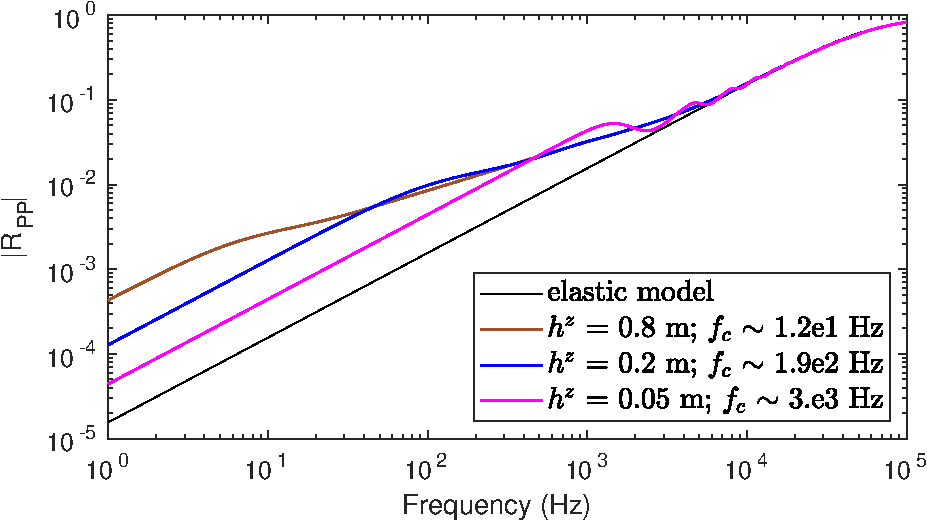
\includegraphics[width=73mm, height=43
       mm]{figures/elasporo_1mm_hsen_k1e-1d.pdf}
        %\label{}
        }
    \subcaptionbox{}
      {
        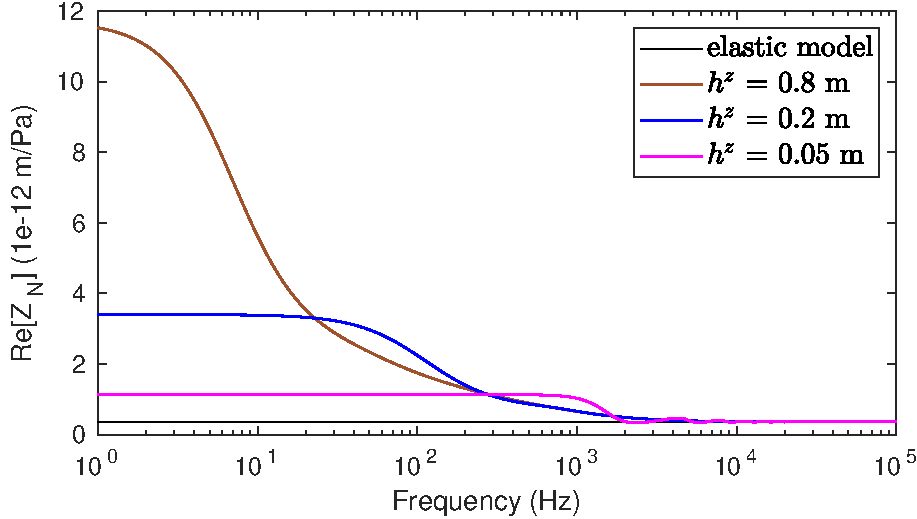
\includegraphics[width=73mm, height=43mm]{figures/elasporo_1mm_hzsen_k1e-1d.pdf}
        %\label{}
        }
\caption {Plots generated using a DZ permeability of 0.1 D and different DZ thicknesses $h^z$. (a) Absolute value of normal P-wave reflectivity $|R_{PP}|$ as a function of frequency. (b) Real part of normal fracture compliance $Z_N$ as a function of frequency}
\label{fig:4}
\end{figure}

\begin{figure}
\centering
    \subcaptionbox{}
      {
       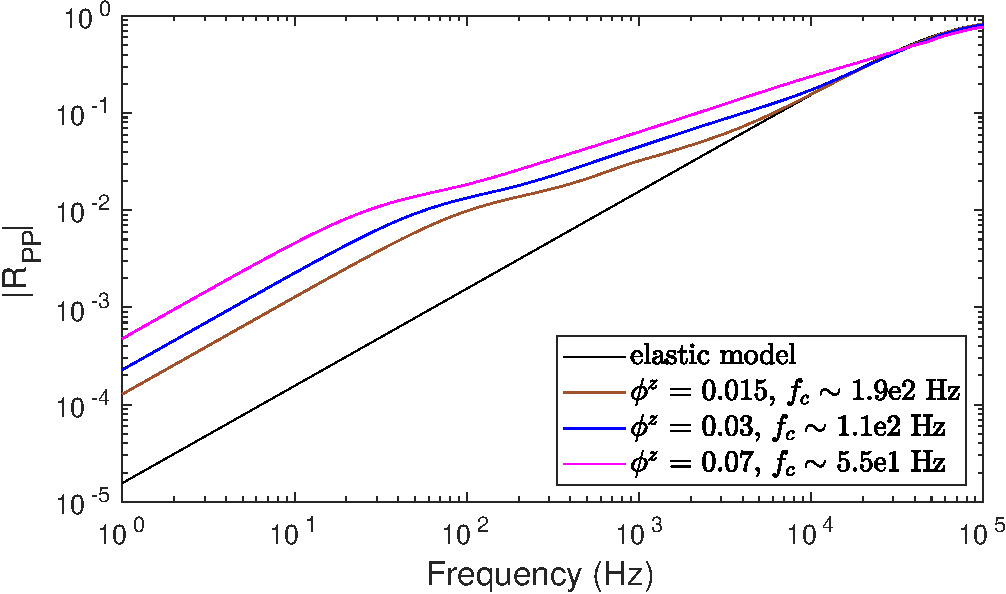
\includegraphics[width=73mm, height=43 mm]{figures/rt_dz_modphi_perm1e-1d.pdf}
        %\label{}
        }
    \subcaptionbox{}
      {
        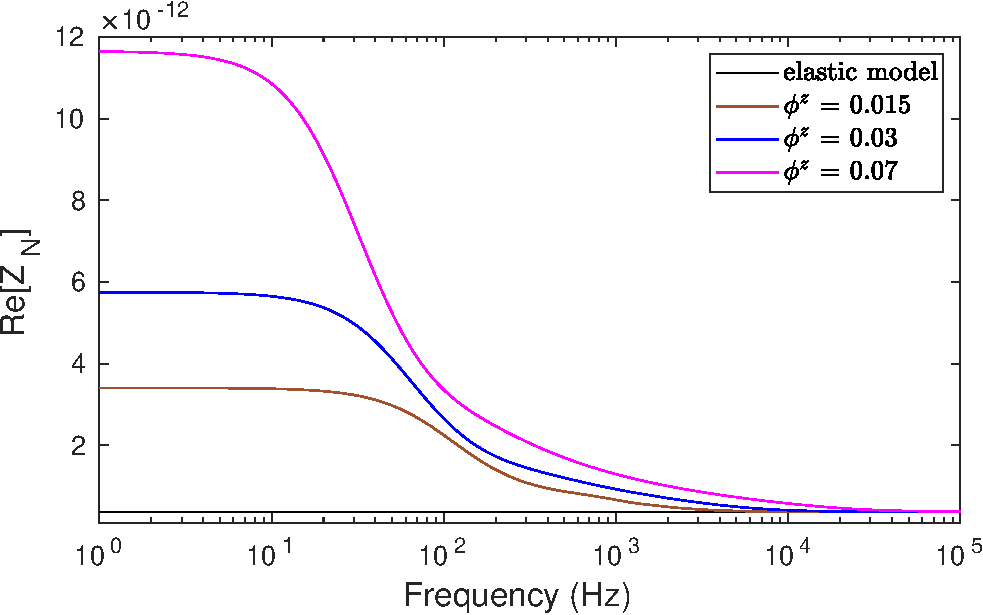
\includegraphics[width=73mm, height=43mm]{figures/zn_dz_modphi_perm1e-1d.pdf}
        %\label{}
        }
\caption {Plots generated using a DZ permeability of 0.1 D and different DZ porosities $\phi^z$. (a) Absolute value of normal P-wave reflectivity $|R_{PP}|$ as a function of frequency. (b) Real part of normal fracture compliance $Z_N$ as a function of frequency}
\label{fig:5}
\end{figure}

\subsection{Effect of fracture moduli}
Figures \ref{fig:6}a and \ref{fig:7}a show the effect of fracture thickness on reflectivity and normal compliance. However, as we  explain in the following, this is equivalent to studying the effect of fracture moduli since both fracture thickness and its moduli are related by equation (\ref{Eq.24}). 
Specifically, Figures \ref{fig:6} and \ref{fig:7} show the effect of two fracture thicknesses, \num{5e-3} m and \num{2e-4} m, respectively, on reflectivity and normal fracture compliance. To find the corresponding bulk and shear moduli, we use equation (\ref{Eq.24}), keeping  $Z_T^d$ and $Z_N^d$ constant. For the fracture with a  thickness of \num{5e-3} m, the corresponding values for $K_m$ and $\mu$ are 0.02 GPa and 0.01 GPa. Similarly, for the fracture  with a thickness of \num{2e-4} m, the corresponding values for $K_m$ and $\mu$ are  \num{8e-4} GPa and  \num{4e-4} GPa. When comparing the corresponding elastic reflectivities $|R_{PP}|$ in Figures \ref{fig:6}a and \ref{fig:7}a, we find that it is higher for the thicker fracture Figure \ref{fig:6}a. However, the maximum increase of reflectivity due to FPD effects is higher for the thinner fracture. This increase for the thinner fracture is more than one-order-of magnitude (Figure \ref{fig:7}a) compared to close to one-tenth of one-order-of magnitude for the thicker fracture (Figure \ref{fig:6}a). 
A similar trend is also evident from the corresponding fracture compliance plots in Figures \ref{fig:6}b and \ref{fig:7}b, with a larger increase of maximum normal compliance for the thinner and softer fracture. In fact, we find that the  $Z_N^o/Z_N^u$ ratios are 2.67 and 43.35 for the thicker and thinner fracture, respectively. We also remark that the transition frequencies are the same as the ones shown in Figure \ref{fig:2} since we have not modified the properties of the DZ.

\begin{figure}
\centering
    \subcaptionbox{}
      {
       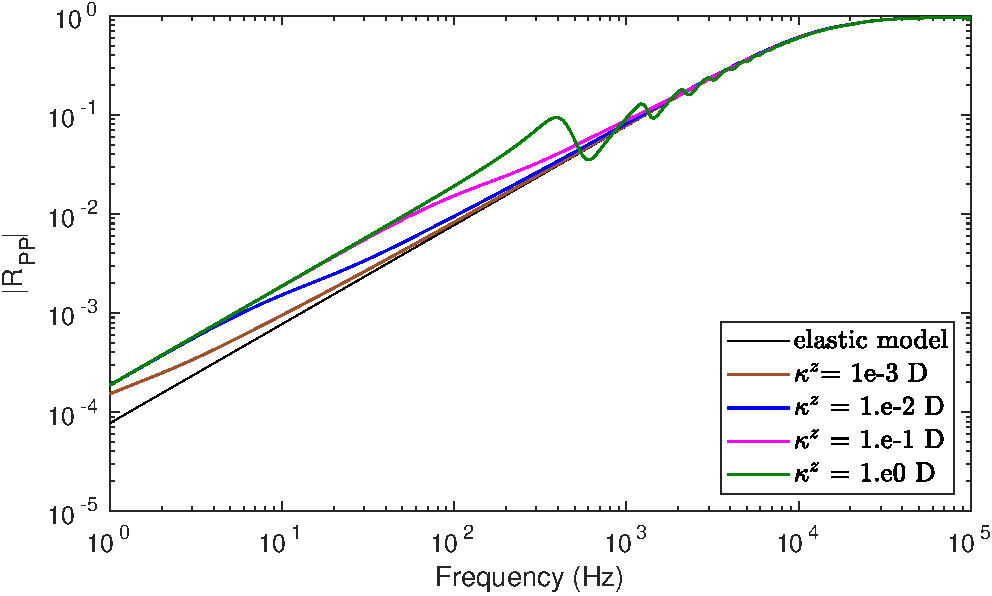
\includegraphics[width=73mm, height=43 mm]{figures/elasporo_5mm_ksen_h20e-2.pdf}
        %\label{}
        }
    \subcaptionbox{}
      {
        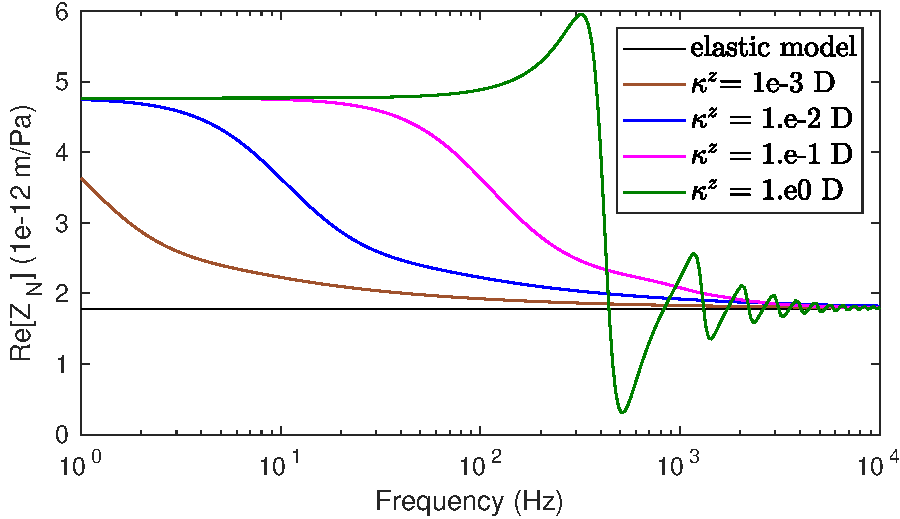
\includegraphics[width=73mm, height=43mm]{figures/elasporo_5mm_znsen_h20e-2.pdf}
        %\label{}
        }
\caption {Plots for a fracture with a thickness of 5.e-3 m. (a) Absolute value of normal P-wave reflectivity $|R_{PP}|$.(b) Real part of normal fracture compliance $Z_N$ as a function of frequency for different DZ permeabilities $\kappa^z$.
}
\label{fig:6}
\end{figure}

\begin{figure}
\centering
    \subcaptionbox{}
      {
       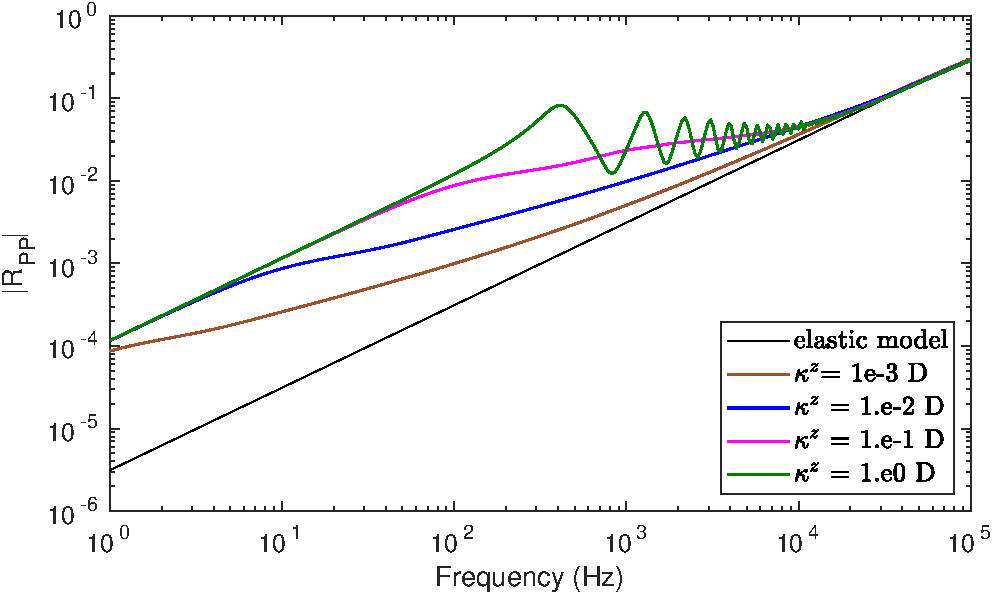
\includegraphics[width=73mm, height=43 mm]{figures/elasporo_02mm_ksen_h20e-2.pdf}
        %\label{}
        }
    \subcaptionbox{}
      {
        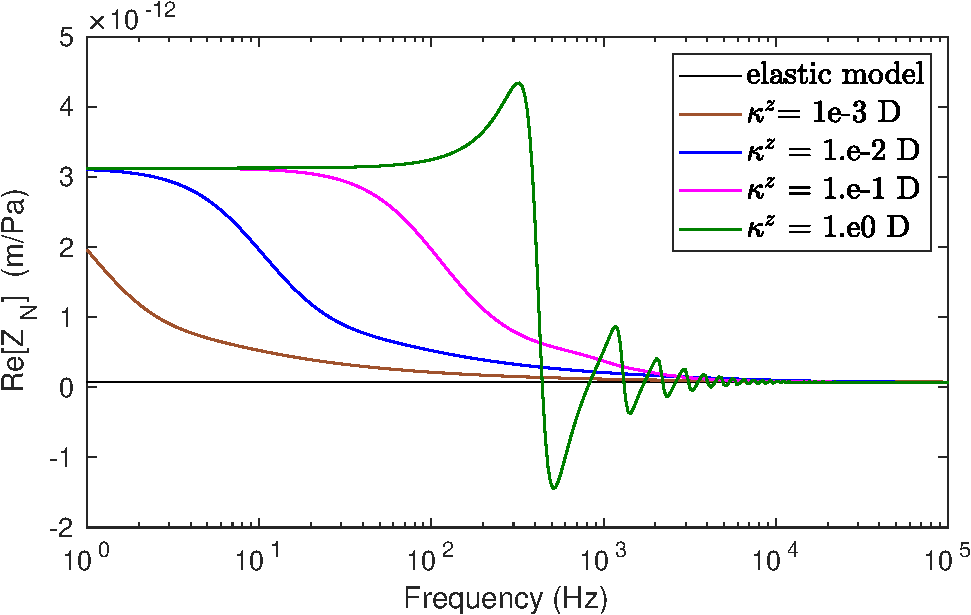
\includegraphics[width=73mm, height=43mm]{figures/elasporo_02mm_znsen_h20e-2.pdf}
        %\label{}
        }
\caption {Plots for a fracture with a thickness of 2.e-4 $m$. (a) Absolute value of normal P-wave reflectivity $|R_{PP}|$. (b) Real part of normal fracture compliance $Z_N$ as a function of frequency for different DZ permeabilities $\kappa^z$.}
\label{fig:7}
\end{figure}

\subsection{Effect of DZ moduli}
In this section, we study the effect of decreasing the drained bulk ($K_m$) and shear ($\mu$) moduli of the DZ and background on reflectivity and normal fracture compliance. Properties for the reference elastic model and elastic-poroelastic model are taken from Table \ref{table:1}. For all elastic-poroelastic models, the background has the same rock properties of the DZ.
For this example  (Figure \ref{fig:8}), we consider the decrease of the reference $K_m^z$ (Table \ref{table:1}) to 19.8 GPa and 6.6 GPa, corresponding to  60\%  and 20\% of its original value, respectively,  while keeping a fixed $K_m^z/\mu^z$ ratio of 1.14. This ratio corresponds to that of the reference moduli.
Solid-line curves in Figure \ref{fig:8}a shows  $|R_{PP}|$ as a function of frequency for a DZ permeability $ \kappa^z $ of 0.1 D and varying values of DZ $K_m^z$. Dashed-lines curves refer to the plots for the corresponding elastic models.
Figure \ref{fig:8}b shows the real part of $Z_N$ for the same DZ parameters. Notice that reflectivity of the elastic models decrease with the bulk modulus of the background (Figure \ref{fig:8}a). This effect is the result of the lower impedance  contrast between the background and the embedded fracture produced by the decreasing values of background moduli. On the other hand, the maximum increase of reflectivity due to FPD does not present such a  monotonic trend.
For a  $K_m^z$ moduli of 19.8 GPa, there is not appreciable difference in the maximum increase of reflectivity when compared to the  reference case ($K_m^z$ = 33 GPa). On the contrary, for a  $K_m^z$ moduli of 6.6 GPa, it is evident that the maximum increase of reflectivity is much lower than for the other two cases. Regarding the impact on normal fracture compliance, Figure \ref{fig:8}b shows that decreasing moduli  results in a greater maximum increase of normal fracture compliance, which is an opposed effect to that on reflectivity (Figure \ref{fig:8}a). This happens because  the decrease of moduli has opposite effects on FPD and impedance ($\rho V_P$), respectively. Figure \ref{fig:8}b indicates that the decrease of moduli promotes FPD, which, in turn, has a positive impact on the maximum increase of normal fracture compliance and therefore, it would have the same positive influence in the maximum increase of reflectivity. However, results of Figure \ref{fig:8}a, reveal that the positive effects of FPD are counteracted by those of an increasingly lower impedance contrast between the background and the fracture-DZ system. In particular, we observe that for the case of using a $K_m^z$ modulus of 19.8 GPa, both effects compensate each other and there is no visible net impact on reflectivity but when the $K_m^z$ modulus is further decrease to 6.6 GPa, the impact of the lower impedance contrast is greater and, therefore, the maximum increase of reflectivity is much lower than the one predicted by FPD effects \ref{fig:8}b.

\begin{figure}
\centering
    \subcaptionbox{}
      {
       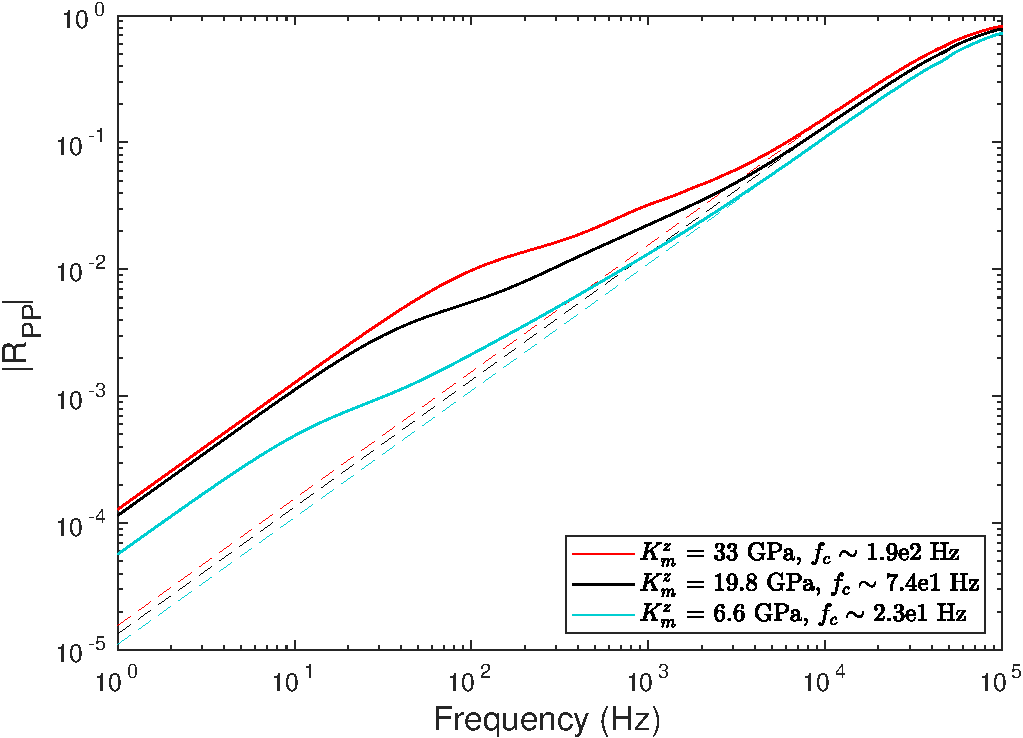
\includegraphics[width=73mm, height=43 mm]{figures/rt_dz_mod_perm1e-1d.pdf}
        %\label{}
        }
    \subcaptionbox{}
      {
        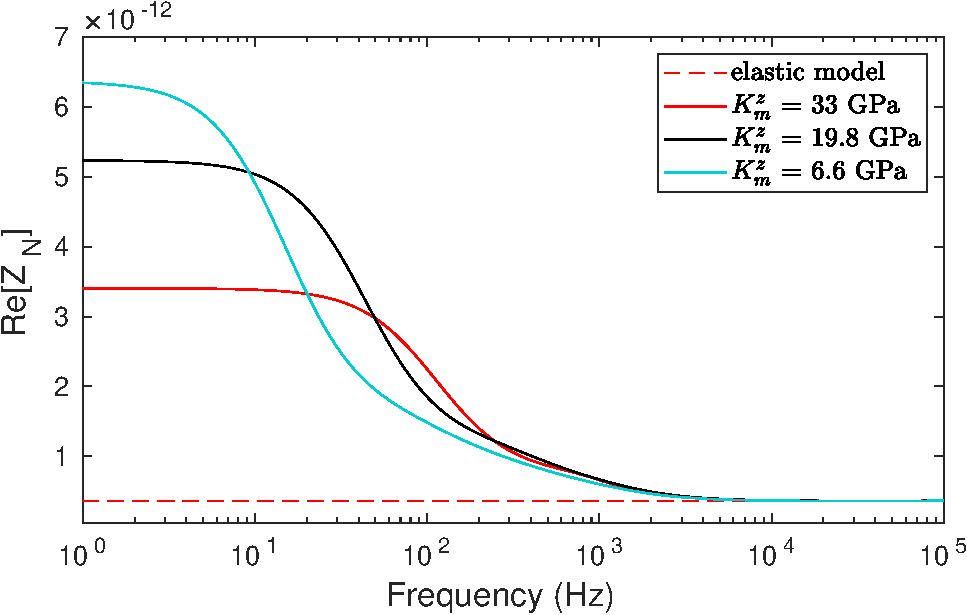
\includegraphics[width=73mm, height=43mm]{figures/zn_dz_mod_perm1e-1d.pdf}
        %\label{}
        }
\caption {Plots with solid lines generated using a DZ permeability of 0.1 D and different DZ  $K_m^z$ moduli with $K_m^z/\mu^z$ ratio of 1.14. For all elastic-poroelastic models, the background has the same rock properties of the DZ. Dashed-line curves denote the corresponding elastic models. (a) Absolute value of normal P-wave reflectivity $|R_{PP}|$ as a function of frequency. (b) Real part of normal fracture compliance $Z_N$ as a function of frequency}
\label{fig:8}
\end{figure}

% \begin{figure}
% \centering
%     \subcaptionbox{}
%       {
%       \includegraphics[width=73mm, height=43 mm]{figures/rt_dz_modratio_perm1e-1d.pdf}
%         %\label{}
%         }
%     \subcaptionbox{}
%       {
%         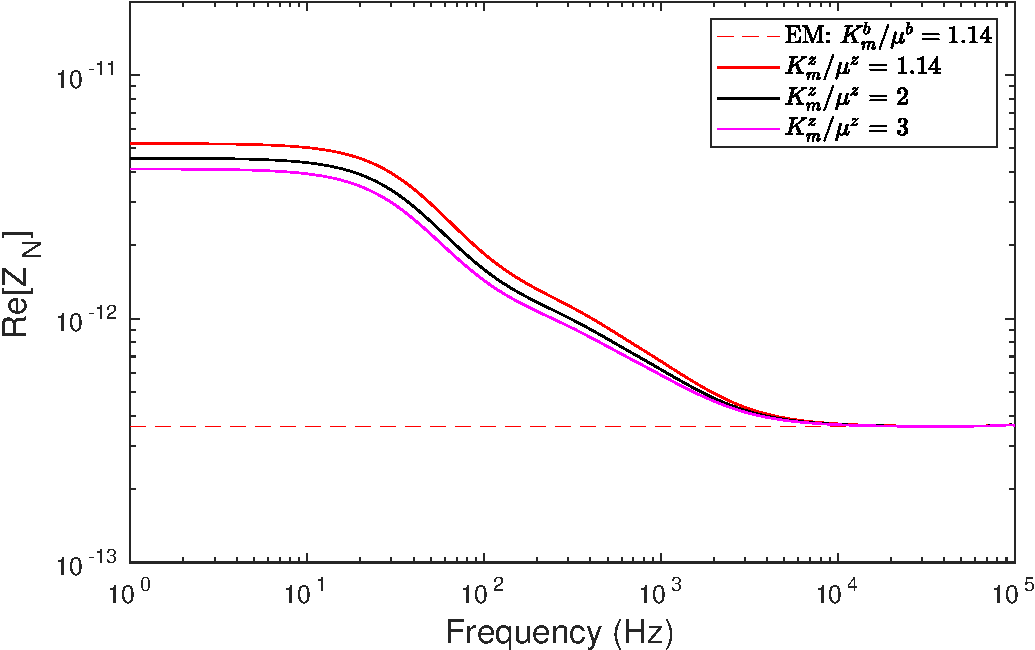
\includegraphics[width=73mm, height=43mm]{figures/zn_dz_modratio_perm1e-1d.pdf}
%         %\label{}
%         }
% \caption {Plots generated using a DZ permeability of 0.1 D and different DZ  $Km^z/ \mu^z$ ratios, with $K_m$ = 19.8 GPa. For all E-PEM, the background has the same rock properties of the DZ. (a) Absolute value of normal P-wave reflectivity $|R_{PP}|$ as a function of frequency. (b) Real part of normal fracture compliance $Z_N$ as a function of frequency}
% \label{fig:9}
% \end{figure}

% \subsection{Effect of a higher porosity and lower moduli of the DZ}
% In the following example, we study the effect of a rock that presents a higher porosity of 0.05 and whose stiffness tensor is characterized by a vertical transverse isotropy (VTI) with softer moduli compared to the reference rock properties of table \ref{table:1} (Figures \ref{fig:8} and \ref{fig:9}). We assign this higher porosity and softer moduli to both the DZ and the elastic background.
% This case emulates a formation whose bedding planes are parallel (Figure \ref{fig:8}) or perpendicular to the fracture plane (Figure \ref{fig:9}). As shown in Figure \ref{fig:2}, it is expected that the higher porosity, compared to the reference case (Figure \ref{fig:3}), further increases the the maximum normal fracture compliance, thus increasing the reflectivity of the system as well. We should also observe the effect on reflectivity of the ratio between the drained bulk modulus and shear modulus since we are using two different sets of moduli. For the results shown in Figure \ref{fig:8},  we assume that the axis of symmetry is parallel to the direction of wave propagation, hence we use softer moduli compared to those for the case when 
% the axis of symmetry is orthogonal to the direction of wave propagation (Figure \ref{fig:9}). 
% %We also investigate the effect of using a different set of rock properties for the DZ and elastic half-spaces.
% %  Figures \ref{fig:8} and \ref{fig:9} present  the reflectivity and normal compliance results after
% % using rock properties for the DZ and elastic background that correspond to a shale formation exhibiting a vertical transverse isotropy (VTI). Thus, for each figure we use different sets of rock moduli to represent two different orientations of the axis of symmetry with respect to the direction of wave propagation. Specifically, 
% %This examples may correspond to a shale formation whose bedding planes are parallel to the fracture plane (Figure \ref{fig:8}) and perpendicular to it (Figure \ref{fig:9}), respectively.
% For Figure \ref{fig:8}, we set $K_m$ and $\mu$ to 15.8 GPa and 5 GPa, respectively, which yields  $r$ = $K_m/\mu$ ratio of 3.2 and  $\bar {H}_d^z (r)$ = 79.
% while for Figure \ref{fig:9} the corresponding moduli are 20.6 GPa and 9.6 GPa, with  $r$ = $K_m/\mu$ ratio of 2.1 and $\bar {H}_d^z (r)$ = 103. We have taken these values from \citeA{Hornby1998}, which are estimations from phase velocities measured at different directions. 
% %The corresponding Thompsen's parameters \cite{Thomsen1986} are: $\xi$ = 0.24 and $\gamma$ = 0.46, which characterizes the medium as weakly anisotropic.
% Additionally, we have set the grain density to 2650 Kg/m$^3$ for both the DZ and half-spaces. We have also used this same grain density for the fracture layer.  We notice that Figure \ref{fig:9} shows a slightly higher increase of reflectivity  and normal fracture compliance than the corresponding plots in Figure \ref{fig:8}. In fact, we find that the ratio $Z_N^o/Z_N^u$ is slightly higher for results in Figure \ref{fig:9}b (26.5) compared to Figure \ref{fig:8}b (25.7). As already mentioned,  this is the consequence of the lower $k_m/\mu$ ratio, 2.1 compared to 3.2, used for the calculations in Figure \ref{fig:9}. This agrees with results of Figure \ref{fig:2}, which shows that, when $\bar {H}_d^z (r)$ values lays on the quasi-constant part of the curve ($\bar {H}_d^z (r)$ between 10 and 100), the impact of the moduli ratio is more important than that of their individual values.
% On the other hand, when we compare reflectivity  against the results obtained with the reference parameters (Figure \ref{fig:3}), we observe that Figures \ref{fig:8}a and \ref{fig:9}a exhibit a lower reflectivity for the elastic curve but they show a higher increase of reflectivity for the elastic-poroelastic cases. According to Figure \ref{fig:2}, this is mainly explained  by the higher porosity considered for the VTI medium (0.05) compared to  that of the reference case (0.015). This effect is also evident from the corresponding $Z_N^o/Z_N^u$ ratios which are  more than two times higher than for the reference results (Figure \ref{fig:4}a). In this case, 
% variations in DZ moduli do not have a major impact  on the increase of reflectivity. This is because, according to Figure \ref{fig:2},
% the effect on the $Z_N^o/Z_N^u$ ratio of $\bar {H}_d^z (r)$ values laying on the quasi-constant part of the curve, as the ones used for the VTI medium, is similar to the effect produced by the  higher ${H}_d^z (r)$ of 165 with a lower moduli ratio $r$ of 1.1 used for the reference case.

% \begin{figure}[hp]
% \centering
%     \subcaptionbox{}
%       {
%       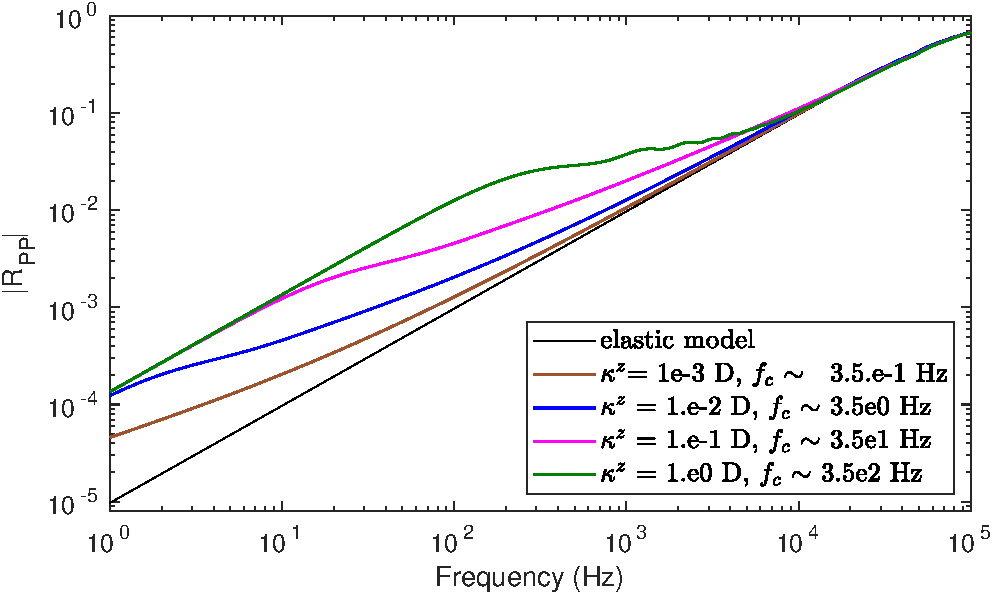
\includegraphics[width=73mm, height=43 mm]{figures/elasporo_1mm_shalev_ksen_h20e-2.pdf}
%         %\label{}
%         }
%     \subcaptionbox{}
%       {
%         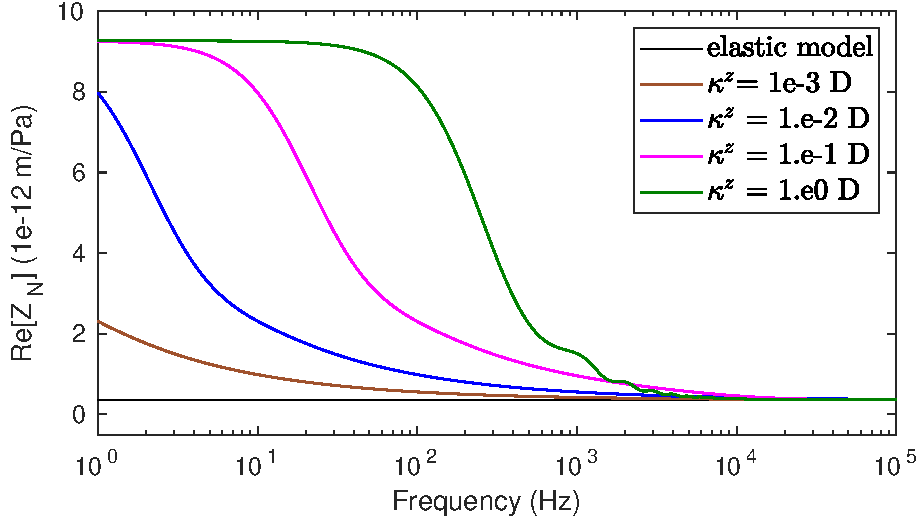
\includegraphics[width=73mm, height=43mm]{figures/elasporo_1mm_shalev_znsen_h20e-2.pdf}
%         %\label{}
%         }
% \caption {Plots considering a VTI medium for the DZ and the elastic background with its  symmetry axis parallel to the direction of wave propagation. (a) Absolute value of normal P-wave reflectivity $|R_{PP}|$. 
% (b) Real part of normal fracture compliance $Z_N$ as a function of frequency for different DZ permeabilities $\kappa^z$.}
% \label{fig:8}
% \end{figure}

% \begin{figure}[hp]
% \centering
%     \subcaptionbox{}
%       {
%       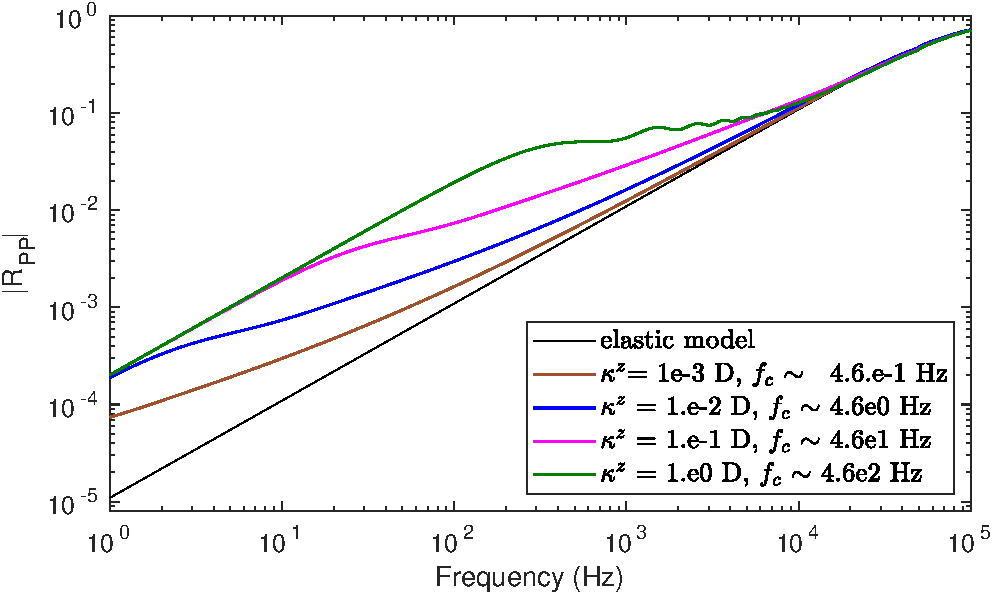
\includegraphics[width=73mm, height=43 mm]{figures/elasporo_1mm_shaleh_ksen_h20e-2.pdf}
%         %\label{}
%         }
%     \subcaptionbox{}
%       {
%         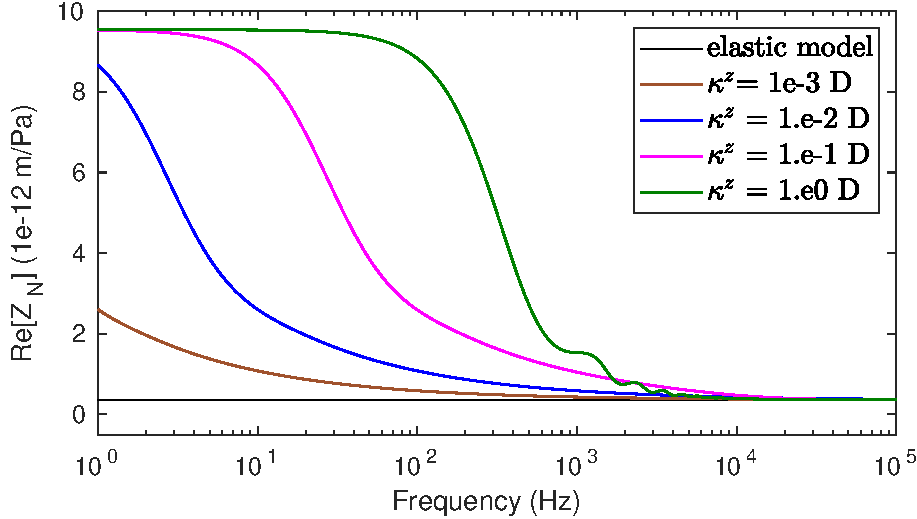
\includegraphics[width=73mm, height=43mm]{figures/elasporo_1mm_shaleh_znsen_h20e-2.pdf}
%         %\label{}
%         }
% \caption {Plots considering  a VTI medium for the DZ and the elastic background with its symmetry axis orthogonal to the direction of wave propagation. (a) Absolute value of normal P-wave reflectivity $|R_{PP}|$. 
% (b) Real part of normal fracture compliance $Z_N$ as a function of frequency for different DZ permeabilities $\kappa^z$.}
% \label{fig:9}
% \end{figure}

\subsection{Effect of a more compressible and less viscous pore fluid in the DZ and fracture}
Next, we study the effect of a more compressible and less viscous fluid filling the pores of the fracture and the associated DZ, such as CO$_2$ (Figure \ref{fig:9}). For the elastic reference model we consider that only the fracture is saturated with
CO$_2$. Although  we have a DZ that does not present the same fluid properties as the impermeable background, we find that at the high frequency limit the elastic impedance reduction is less than 1 \%, when considering  supercritical CO$_2$ as the saturating fluid in the DZ instead of water. This negligible effect of supercritical CO$_2$ occurs because the moduli of the drained bulk frame and of the grains in the DZ have
comparable values. This, in turn, leads to a very small Biot-Willis coefficient $\alpha$ $\sim$ 0.1, rendering the fluid effect imperceptible when evaluating the undrained Lamé parameter $\lambda$ and, therefore, the velocity of the medium (equations \ref{Eq.3} and \ref{Eq.12}), regardless of the fluid type.
Thus, in the high-frequency limit, both the elastic-poroelastic and purely elastic models present the same seismic response for practical purposes. For our analysis, this is desirable since we are preferentially showing the effects of FPD.
We remark that this is also the consequence of using the same mechanical properties for both the DZ and the background. However, it is expected that the DZ presents softer moduli compared to the background and thus, produces a higher impedance contrast, with observable fluid effects. The presence of supercrital CO$_2$ in the fracture and DZ could be the result of an injection process \cite{Lumley2010}. 
Although, a complete saturation of the pores with CO$_2$ is not realistically expected \cite{Chadwick2005,Chadwick2010}, this simplification captures the main changes produced by a fluid that is less viscous and more compressible on fracture compliance and reflectivity of the system. 
We set the supercritcal CO$_2$ properties $K_f$, $\rho_f$ and $\eta$ to 0.0229 GPa, 693 Kg/m$^3$ and \num{1.56e-5} Pa.s, respectively. These values are taken from \citeA{Rubino2011}. 
Reflectivity results (Figure \ref{fig:9}a) show that the elastic reflectivity  is close to two-orders-of magnitude higher than that obtained using water as the saturating fluid (Table \ref{table:1} and Figure \ref{fig:2}). However, the maximum increase of reflectivity due to FPD  is less pronounce. Figure \ref{fig:9}a shows a maximum reflectivity increase of less than half of an order-of-magnitude, while the same results with water as saturating fluid show a maximum reflectivity increase close to one order-of-magnitude (Figure \ref{fig:2}).
A similar trend is observed for the normal fracture compliance, with  higher values for the elastic normal compliance, of order of \num{1e-11} m/Pa, for the fracture-DZ system with supercritical CO$_2$ as saturating fluid (Figure \ref{fig:9}b) than for the reference case with water as the saturating fluid, which is characterized by an elastic compliance of order of \num{1e-12} m/Pa (Figure \ref{fig:3}a). Nonetheless, the maximum increase of compliance due to FPD effects is less for the case of CO$_2$ as saturating fluid, as indicated by its lower  $Z_N^o/Z_N^u$ ratio of 3.51 compared to the case of  water as  saturating fluid, with a higher $Z_N^o/Z_N^u$ ratio of 9.45.
For the case of CO$_2$ as saturating fluid, lower maximum values of compliance and reflectivity due to FPD happen because this high compressible fluid prevent a significant increase of fluid pressure inside the fracture despite of being heavily deformed. Therefore, the fluid pressure gradient between the fracture and the DZ is small, and so are the FPD effects.
Another effect of considering supercritical CO$_2$ as the pore fluid is the decrease of the transition frequency $f_c$ for a given DZ permeability, which is around 10 \% with respect to the water-saturated case. This is the result of the higher impact of the reduction of  fluid compressibility compared to the impact of the decrease of its viscosity (Equations \ref{Eq.19} and \ref{Eq.21}). We also observe the earlier onset of reverberations in Figure \ref{fig:9} than for the reference case (Figures \ref{fig:2} and \ref{fig:3}a ) for the curves corresponding to DZ permeabilities of 1 D and \num{1 e-1} D, respectively. This is consequence of much lower values of Biot's frequency for the DZ: $\sim$ \num{1.8e1} Hz and $\sim$ \num{1.8e2} Hz, respectively, caused by the lower fluid viscosity.

\begin{figure}[hp]
\centering
    \subcaptionbox{}
      {
       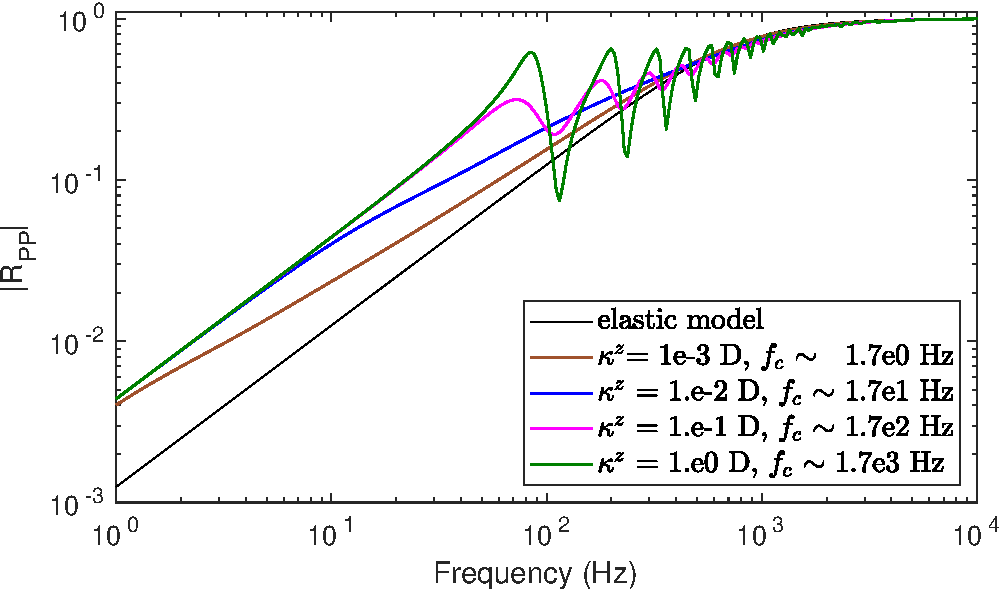
\includegraphics[width=70mm, height=43 mm]{figures/elasporo_1mm_co2fdz_ksen_h20e-2.pdf}
        %\label{}
        }
    \subcaptionbox{}
      {
        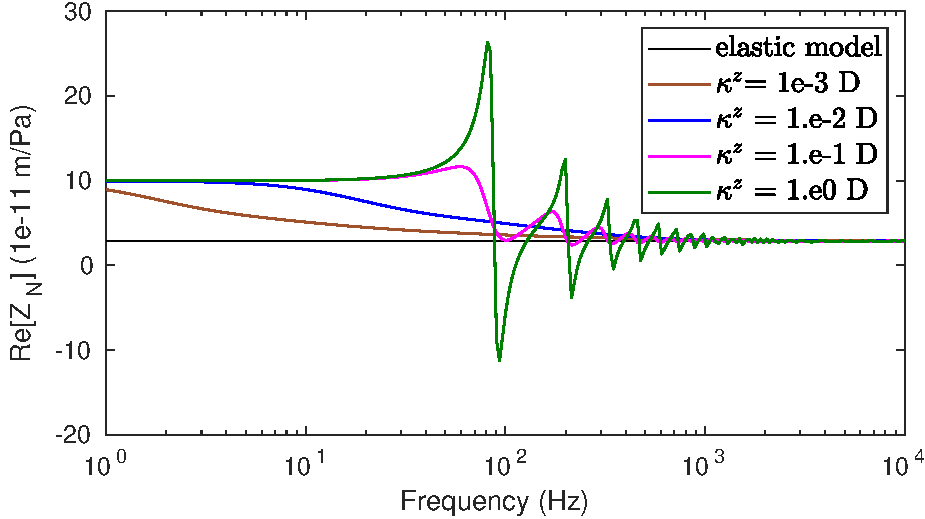
\includegraphics[width=73mm, height=43mm]{figures/elasporo_1mm_co2fdz_znsen_h20e-2.pdf}
        %\label{}
        }
\caption {Plots considering  CO$_2$ in supercritical state as the saturating pore fluid for the fracture and associated DZ.
(a) Absolute value of normal P-wave reflectivity $|R_{PP}|$. (b) Real part of normal fracture compliance $Z_N$ as a function of frequency for different DZ permeabilities $\kappa^z$. }
\label{fig:9}
\end{figure}

\subsection {Sensitivity analysis of the maximum increase of normal fracture compliance}

We have shown in the previous examples the effect of discrete variations of rock and fluid properties of the DZ and fracture on the maximum increase of fracture normal compliance. In this section we investigate in more detail the sensitivity of the maximum increase of fracture normal compliance to the  changes of rock and fluid properties. These properties are changed at a time while keeping the other ones constant and equal to the values shown in Table \ref{table:1}.
% We perform this because FPD in its has a direct effect on the maximum increase of fracture normal compliance, 
We let the $Z_N^o/Z_N^u$ ratio be a measure of the maximum increase of fracture normal compliance due to FPD. According to equation (\ref{Eq.23}), $Z_N^o$ is the low-frequency limit of normal compliance of the fracture, meaning that it is the maximum value that it can take because at this frequency limit FPD is on its relaxed regime,  causing that the largest possible volume of fluid exits the fracture. This, in turn, decreases to a minimum the fluid stiffening effect in the fracture. In contrast, $Z_N^u$ is the high-frequency limit of normal compliance of the fracture, indicating that this is the lowest value that it can take because at this frequency limit the unrelaxed FPD regime prevails producing that the fracture behaves as hydraulically isolated. At this stage, the normal compliance value is that of an elastic fracture. Therefore, the  $Z_N^o/Z_N^u$ ratio provides a measure of the maximum increase of normal fracture compliance due to FPD  with respect to its elastic limit. To show how this maximum increase is controlled by the rock and fluid properties, we plot the $Z_N^o/Z_N^u$ ratio as a function of dimensionless properties $X$ (Figure \ref{fig:10}), where $X$ indicates the times a reference property value has increased. The different dimensionless properties that $X$ represent are: the increment of the fracture bulk modulus $\bar{K}_m^c$, the increment of the DZ bulk modulus $\bar{K}_m^z $, the increment of the DZ thickness $\bar{h}^z$ and the increment of the fluid bulk modulus $\bar{K}_f$. We indicate that $\phi^z$ is not a dimensionless variable but is the porosity of the DZ expressed in percentage. The corresponding reference values are: the bulk modulus of the fracture and DZ $\tilde{K}_m^c$ = \num{4e-4} GPa and $\tilde{K}_m^z$ = 0.2 GPa, respectively, the DZ thickness $\tilde{h}^z$ = 0.01 m and the fluid bulk modulus $\tilde{K}_f$ = 0.01 GPa.
We remark that the response of $Z_N^o/Z_N^u$ ratio to the variations $\bar{K}_m^c$ and $\bar{K}_m^z$ includes as well the effect of the respective shear moduli changes. Nonetheless, for the figure,  we only show the values that the dimensionless bulk moduli take.
For the case of the fracture, we find the both the bulk and shear modulus by means of equation (\ref{Eq.24}). To this end, we vary the thickness of the fracture from \num{e-4} m to \num{e-2} m, while keeping constant the tangential and drained normal compliance to \num{5e-10} m/Pa and \num{1.5e-10} m/Pa, respectively. Then, the reference modulus $\tilde{K}_m^c$ correspond to that found with a fracture thickness of \num{e-4} m. For the case of the DZ, we simply assume that the bulk modulus is 1.14 times greater than its shear modulus. This moduli ratio is the same as the one corresponding to the DZ moduli in Table \ref{table:1}. Observe that the increase of most of the dimensionless rock and fluid properties produce a monotonically increase or the decrease of the $Z_N^o/Z_N^u$ ratio. Properties producing an increase of the $Z_N^o/Z_N^u$ as they increment are $\phi^z (\%)$, $\bar{h}^z$ and $\bar{K_f}$. As already investigated in the previous examples, the increase $\phi^z (\%)$, $\bar{h}^z$ has a positive impact on the maximum increase of normal fracture compliance because they provide a greater pore volume for FPD. On the other hand, an increasingly stiffer fluid $\bar{K_f}$, creates the necessary pressure gradient for FPD.
In contrast, the increment of $\bar{K}_m^c$ produces a continuous decrease of the $Z_N^o/Z_N^u$ ratio because the fracture becomes increasingly stiffer. However,  $\bar{K}_m^z$  is the only property, among the ones studied, that do not produce a monotonic response of the  $Z_N^o/Z_N^u$ ratio. We observe that, for sufficiently low values of $\bar{K}_m^z$, the increase of this property causes a continuous rise of  $Z_N^o/Z_N^u$ until a maximum  is reached. Then, a further increase of $\bar{K}_m^z$ produces a continuous decline of the $Z_N^o/Z_N^u$ ratio. In section 3.3, we have partially analyzed the effects of DZ moduli on the maximum increase of fracture normal compliance.
In that analysis we have found that for values of  $K_m^z \geq$ 6.6 GPa ($\bar{K}_m^z \geq$ 33), the maximum increase of normal fracture compliance becomes lower with the increase of  $K_m^z$. This  means that for the $K_m^z$  values used in that section, the response of the $Z_N^o/Z_N^u$  ratio is in the decreasing part of the curve.
Notice that, for this sensitivity analysis, we do not consider neither the permeability of the DZ nor the viscosity of the saturating fluid because, according to equation (\ref{Eq.23}),  none of these properties has any effect on the maximum increase of normal compliance. Nonetheless, these parameters control the transition frequency between FPD regimes (equations (\ref{Eq.19}) and (\ref{Eq.21})).

Table \ref{table:2} shows the $Z_N^o/Z_N^u$  ratios for the rock and fluid properties analyzed in the previous examples. Here, the column \emph{Marker} refers to the marker used in Figure \ref{fig:10} to plot the respective data entry.
These results can be compared against the  $Z_N^o/Z_N^u$ ratio  of 9.45 obtained for the reference elastic-poroelastic model using the properties of Table \ref{table:1}. The  dimensionless variables of interest for the rock and fluid properties of Table \ref{table:1} are: $\bar{h}^z$ = 20, $\bar{K}_m^z$ = 165, $\bar{K}_m^c$ = 10 and $\bar{K}_f^z$ = 225.

\begin{figure}
\centering
     % \subcaptionbox{}
      {
        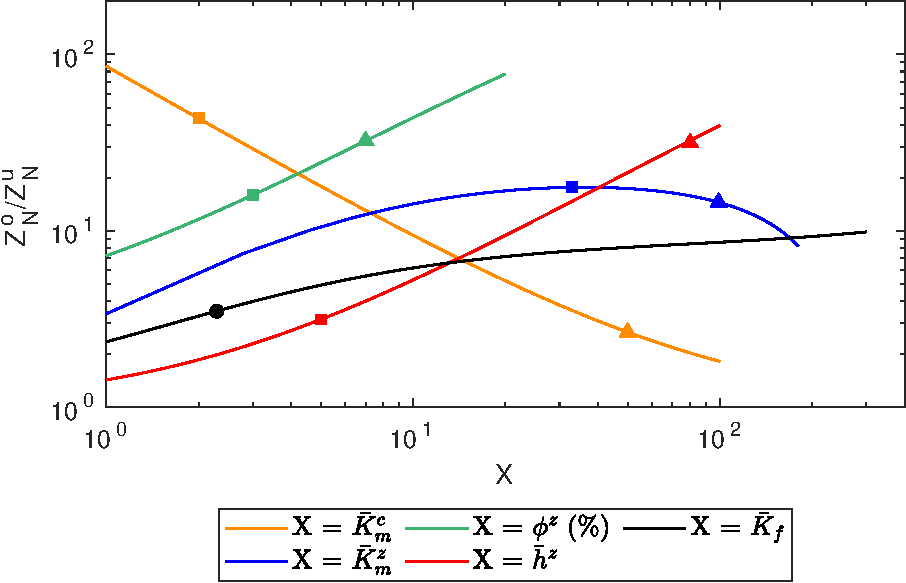
\includegraphics[width=85mm, height=55mm]{figures/zno_znu_sensitivity.pdf}
        %\label{}
        }
        
\caption { $Z_N^o / Z_N^u$ ratio as function of dimensionless rock and fluid parameters $X$. These parameters represent the times a reference value is incremented, except for $\phi^z$ which is the porosity of the DZ expressed in percentage. The corresponding dimensionless parameters are: the increment of the fracture bulk modulus $\bar{K}_m^c$, the increment of the DZ bulk modulus $\bar{K}_m^z$, the increment of DZ thickness $\bar{h}^z$ and the increment of the fluid bulk modulus $\bar{K}_f$. The corresponding reference values are: the bulk modulus of the fracture $\tilde{K}_m^c$ = \num{4e-4} GPa, the bulk modulus of the DZ $\tilde{k}_m^z$ = 0.2 GPa, the thickness of DZ $ h^z$ = 0.01 m and the bulk modulus of th fluid $ K_f$ = 0.01 GPa. Markers denote data points from Table \ref{table:2}.
}
\label{fig:10}
\end{figure}


\begin{table}[!ht]
  \caption{$Z_N^o/Z_N^u$ ratio for the different rock and fluid properties studied in the previous examples}
\begin{center}
  \begin{tabular}{ | l | c | c| c| }
    \hline
    Property (dimensionless) & Property value (dimensionless) & $Z_N^o/Z_N^u$ & Marker \\
    \hline
    \multirow{2}{10em}{$h^z$  $\left( \bar{h}^z \right)$} & 0.05 m (5) & 3.15 & \color{red}\FilledSquare \\ 
     & 0.8 m (80) & 31.51 & \color{red}\FilledTriangleUp \\ 
    \hline
    \multirow{2}{10em}{$\phi^z$  $ \left( \phi^z (\%) \right)$} & 0.03  (3 \%) & 15.96 & \color{green}\FilledSquare\\ 
     & 0.07  (7 \%) & 32.35  & \color{green}\FilledTriangleUp \\ 
     \hline
        \multirow{2}{10em}{$K_m^z$ $ \left( \bar{K}_m^z \right)$} & 6.6 GPa (33) & 17.67 & \color{blue}\FilledSquare \\ 
     & 19.8 GPa (99) & 14.53  & \color{blue}\FilledTriangleUp \\ 
    \hline
     \multirow{2}{10em}{$K_m^c$ $ \left( \bar{K}_m^c \right)$} & \num{8e-4} GPa (2) & 43.35 & \color{orange}\FilledSquare \\ 
     & 0.02 GPa (50) & 2.67 & \color{orange}\FilledTriangleUp \\ 
    \hline
    $K_f$ $\left( \bar{K}_f \right)$  & 0.0229 GPa (2.29) & 3.51 & \color{black}\FilledCircle\\ 
      
    \hline
  \end{tabular}
  \label{table:2}
\end{center}
\end{table}


\subsection{Discussion}
In this work we have shown that the presence of a DZ increases the compliance and reflectivity of the fracture due to FPD. Specifically, our study indicates that the rock and fluid  physical properties of the DZ and fracture  have a direct control of the fluid exchange between these two regions due to FPD and, therefore, they determine the maximum increase of normal fracture compliance from its elastic limit. However, the effect of the same rock properties on reflectivity do not necessary follow the same trend as that on the normal fracture compliance because these properties may have opposite effects on FPD between the fracture and DZ and the impedence contrast between the background and fracture-DZ system. This is, for instance evident, for the case of decreasing moduli of the DZ and background (Figure \ref{fig:8}).



%  we analyze the influence of these properties on the maximum increase of fracture normal compliance from its undrained value due to FPD effects in its relaxed state.
% We define this maximum increase as the ratio  between the low- and high-frequency limits of normal fracture compliance: $Z_N^o/Z_N^u$. The individual terms of this ratio is specified in equation (\ref{Eq.23}). 
% The motivation behind this analysis is to provide an indication of the effect of these same fluid and rock properties on the maximum increase of reflectivity of the poroelastic system compared to the pure elastic model due to FPD effects. In this regard, the ratio  $Z_N^o/Z_N^u$ can provide such an indication because each of these terms, $Z_N^o$ and $Z_N^u$, controls the mechanical contrast between the DZ-fracture system and elastic background at the limiting FPD regimes, relaxed and unrelaxed, repectively and, as a consequence, they constrain the maximum and minimum values of reflectivity due to FPD effects. 
% Specifically, the low-frequency limit of normal fracture compliance $Z_N^o$  restricts the maximum mechanical contrast between the DZ-fracture system and the background. This is the result of FPD effects in its relaxed regime yielding the highest possible normal fracture compliance. Conversely, the high-frequency limit of normal fracture compliance $Z_N^u$ controls the corresponding minimum mechanical contrast. This is because $Z_N^u$  is the lowest possible value of normal compliance as it corresponds to the elastic limit, meaning that the fracture behaves as hydraulically isolated.
% Figure \ref{fig:2} presents the sensitivity of the maximum increase of normal fracture compliance $Z_N^o/Z_N^u$ to the variation of dimensionless rock and fluid properties $X$ as specified in the caption.
% Notice that we present the drained plane-wave modulus to characterize the mechanical properties of the fracture and its associated DZ because it combines the drained bulk and shear moduli, which are the properties that we are in fact modifying. For the fracture, we find $H_d^c$ values by using equation (\ref{Eq.24}) and varying the thickness of the fracture from \num{e-4} m to \num{e-2} m, while keeping constant the compliance values. For the DZ, we vary its bulk modulus $K_m^z$ from 0.2 GPa to 36 GPa. 
% In the figure, observe the effect of the ratio $r_i$ = $K_{m_i}^z/\mu_i^z$: the lower the ratio ( $r_1$ = 1.4 versus $r_2$ = 3) the higher the increase of $Z_N^o/Z_N^u$. This latter effect is relevant in anisotropic rocks in which the ratio of the mechanical moduli may vary according to its stiffness tensor orientation with respect to the direction of wave propagation.
% Notice as well the behavior of the curves for $X$ = $\bar {H}_d^z (r_i)$. They monotonically increase until $\bar {H}_d^z (r_i) \sim$  10, corresponding to $K_{m_i}^z$ = 2 GPa, then they basically present a constant value until $\bar {H}_d^z (r_i) \sim$ 100,  corresponding to $K_{m_i}^z$ = 20 GPa, point at  which they slightly decrease. These observations indicate that  $Z_N^o/Z_N^u$ is not very sensitive to variations $\bar {H}_d^z (r_i)$ unless the rock moduli are relatively low ($K_{m_i}^z$ less than 2 GPa)  or  high ($K_{m_i}^z$ greater than 20 GPa). Commonly, intact rock masses present $K_{m_i}^z$ values between 5 GPa and 33 GPa which correspond to  $\bar {H}_d^z (r_i)$ values between 25 and 165, respectively. On the other hand, the ratio  $Z_N^o/Z_N^u$ shows greater sensitivity to the variation of the drained plane-wave modulus of the fracture $\bar{H}_d^c$ and the thickness of the DZ, ($\bar{h}^z$).


% To summarize the findings of this section, we present Figure \ref{fig:11},  which shows the ratio of the absolute values of normally incident P-wave reflectivity as a function of frequency for the different cases explored above. The respective reflectivities correspond to the elastic-poroelastic model ($|R_{PP}^p|$) and the elastic model ($|R_{PP}^e|$) from the examples previously presented for a DZ permeability of 0.1 D. This ratio provides a measure of the increase of reflectivity  with respect to its corresponding purely elastic case due to FPD effects, reflecting as well the influence of changes in rock and fluid properties.
% The reference model corresponds to the case in which reflectivities are calculated with the rock and fluid properties in Table \ref{table:1}.
% According to this figure, the example with the thinner softer fracture presents the highest increase of reflectivity,  around 13 times that of  the corresponding elastic case. Conversely, the lowest increase of reflectivity, of around 1.5 times, corresponds to the case of the thicker stiffer fracture.
% Regarding the effect of the bulk modulus of the saturating fluid, we observe that for the case  with the more compressible fluid, supercritical CO$_2$, there is a lower increase of reflectivity, a  bit more than two times, compared to the reference model in which water is the saturating fluid. As already explained, this lower increase of reflectivity is due to the high compressibility of  supercritical CO$_2$ that prevents  high pressure gradients for FPD.
% Concerning the effect of different sets of rock properties, we notice that the two curves corresponding to the VTI medium  show a higher increase of reflectivity than for the reference case: between ten to eleven times versus close to eight times. This higher reflectivity for the VTI cases is better explained by the effect of their higher porosity values of 0.05 against 0.015 for the reference model since their softer moduli have no major impact on reflectivity.
% This is because these moduli correspond to the quasi-constant part of the $Z_N^o / Z_N^u$ ratio curve, producing an increase on this ratio that is similar to the one produced by the  moduli from the reference rock properties (Figure \ref{fig:2}). However, the difference in reflectivity between the parallel and transvere cases  is a consequence of the two different $k_m/\mu$ ratios used, with a higher increase of reflectivity for the lower ratio (transverse). Overall these results are in agreement with the analysis of $Z_N^o / Z_N^u$ presented in Figure \ref{fig:2}, which shows a higher ratio as the fracture become softer, corresponding to a higher increase of reflectivity. In constrast, it shows a lower $Z_N^o / Z_N^u$ ratio as the saturating fluid becomes more compressible.

% \begin{figure}[!ht]
% \centering
%         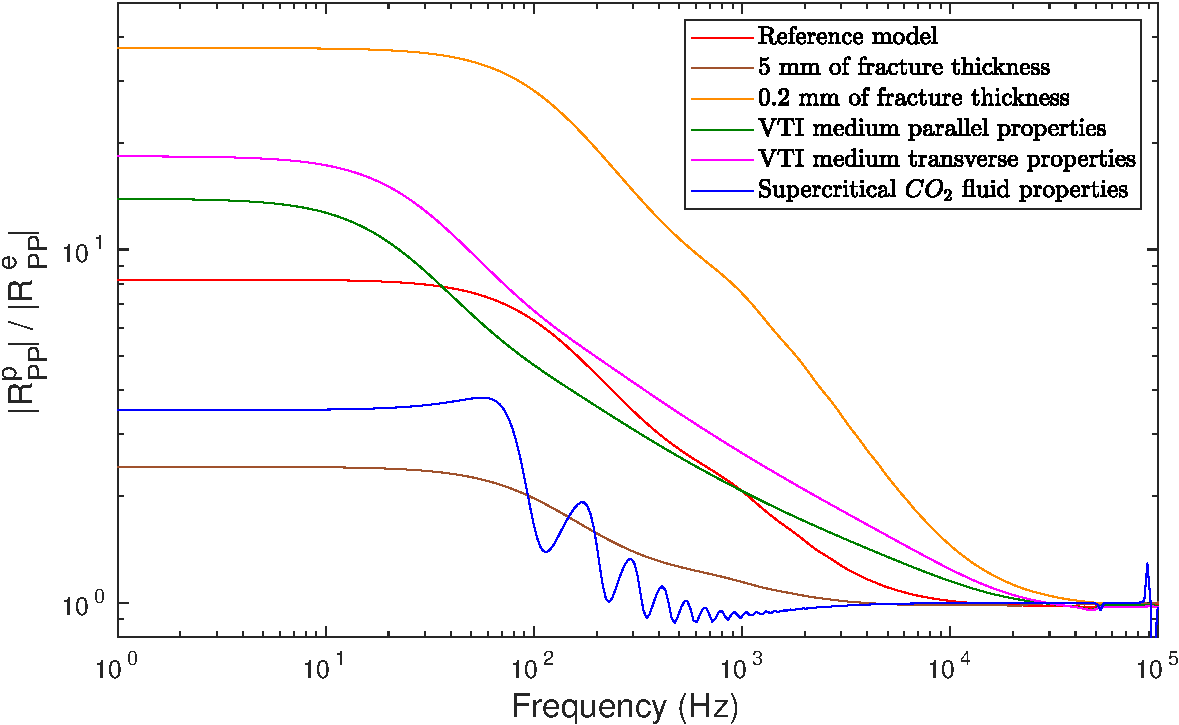
\includegraphics[width=110mm, height=70mm]{figures/ratioRT_elasporo_elas.pdf}
%         %\label{}
% \caption {Ratio of the absolute values of normally incident P-wave reflectivity as a function of frequency, with reflectivities from the elastic-poroelastic model ($|R_{PP}^p|$) and the corresponding elastic model ($|R_{PP}^e|$), respectively, for the examples previously presented for a DZ permeability of 0.1 D. The reference model corresponds to the case for which the rock and fluid properties are those given in Table \ref{table:1}}.
% \label{fig:10}
% \end{figure}

For this work, we  have considered that the DZ and the impermeable background present the same rock properties except for permeability since we  have aimed to highlight mainly the effects of FPD on reflectivity.
Thus, we have not analyzed the effect on reflectivity of any  decrease in mechanical moduli  or increase in porosity in the DZ with respect to the background, although these effects are expected due to the presence of micro- and macro-fractures in the DZ. In Figure \ref{fig:11} we present such analysis. In this figure, solid curves correspond to elastic-poroelastic models for a DZ permeability of 0.1 D and dashed curves of the same color denote the corresponding elastic model. Unless otherwise stated, other DZ properties are the same as in Table \ref{table:1}.
The elastic models include DZ layers (Figure \ref{fig:1}a)
when the DZ rock properties are different from those of the background. For such cases, the reflection coefficient is calculated at the background-DZ interface.
Figure \ref{fig:11}a shows the effect of the decrease of DZ bulk and shear moduli while the background moduli is kept constant and equal to the values of Table \ref{table:1} for the DZ entry. The red solid curve correspond to the elastic-poroelastic model for which the background and DZ present the same rock and fluid properties. The corresponding elastic model (red-dashed curve) does not include DZ layers. (Figure \ref{fig:1}b).
From the plots, we observe that the elastic reflectivities at the background - DZ interface are greater than that obtained at the the background - fracture interface (red-dashed curve). The reason for this increase in reflectivity is the presence of a thicker softer layer comprised by the DZ and fracture that produces a higher impedance contrast with the background, with increasing elastic reflectivity as the DZ becomes thicker and softer. In contrast,  the maximum increase of reflectivity due to FPD from its corresponding elastic reference decreases as the DZ becomes softer. This is the consequence of the decreasing mechanical contrast between the DZ and the fracture. Nonetheless, it is likely that the DZ becomes not only softer but also more porous. Figure \ref{fig:11}b presents reflectivities of models considering  increasing porosities of a DZ that is softer than the background. As expected, the increase of the pore volume promotes FPD, increasing the maximum reflectivity from its elastic reference, thus counteracting the effect of the decrease of DZ moduli.

\begin{figure}[hp]
\centering
    \subcaptionbox{}
      {
       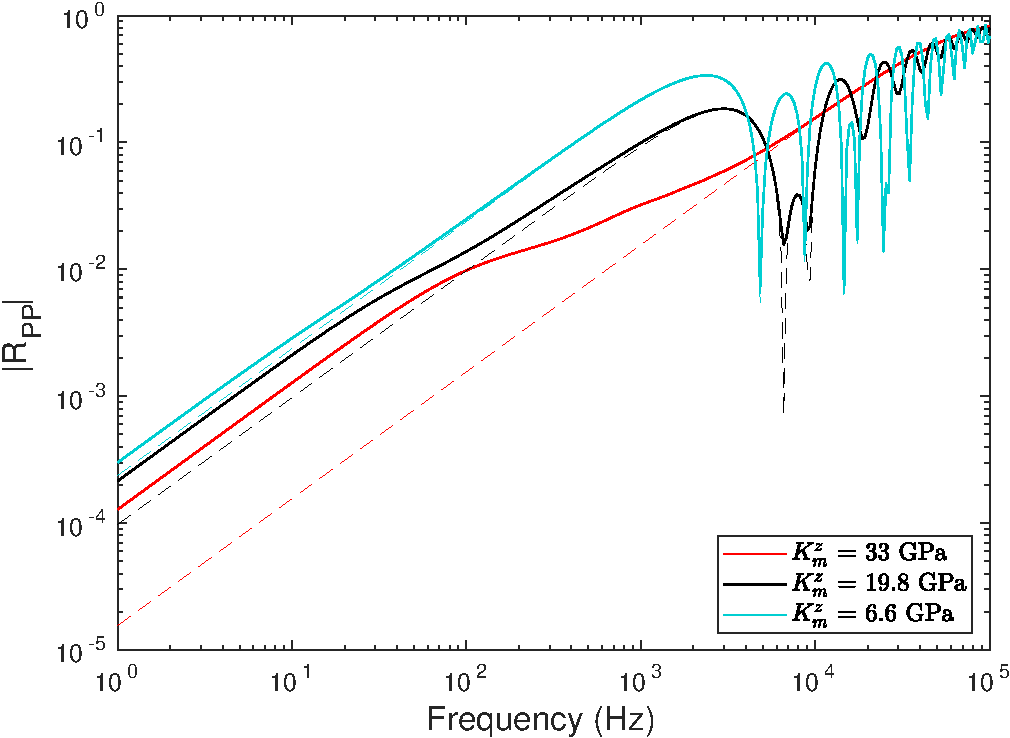
\includegraphics[width=70mm, height=45 mm]{figures/rt_dz_km_perm1e-1d.pdf}
        %\label{}
        }
    \subcaptionbox{}
      {
        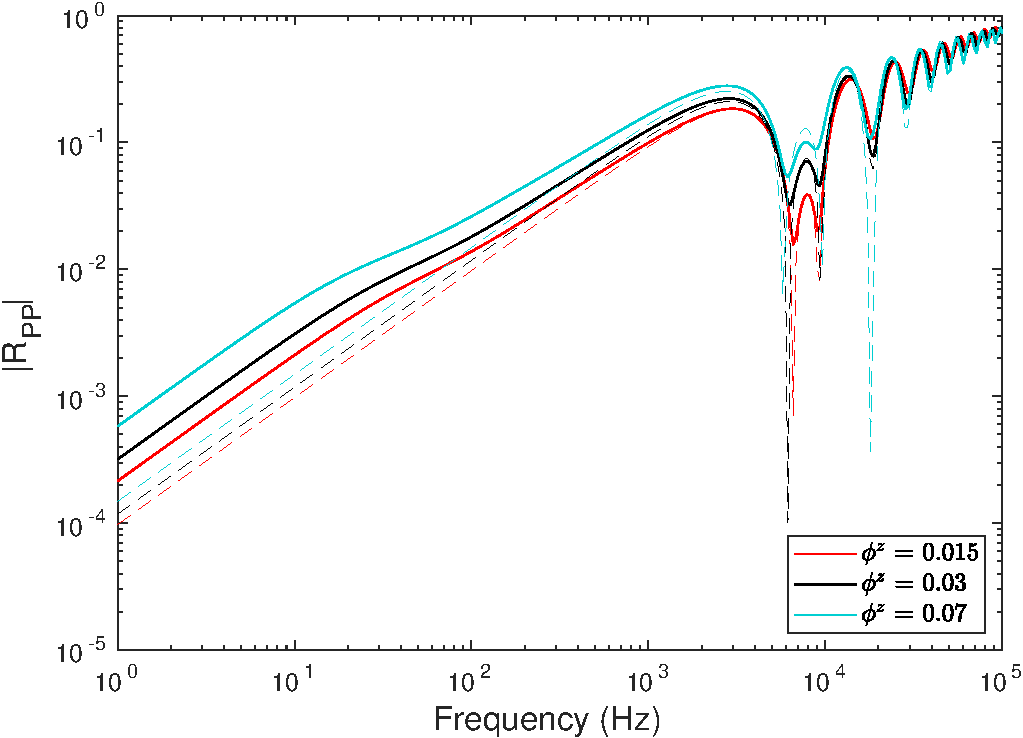
\includegraphics[width=73mm, height=45mm]{figures/rt_dz_kmphi_perm1e-1d.pdf}
        %\label{}
        }
\caption {
 Plots show the absolute value of normal P-wave reflectivity $|R_{PP}|$ as a function of frequency.
 Solid curves correspond to elastic-poroelastic models for a DZ permeability of 0.1 D. Dashed curves of the same color denote the corresponding elastic models. (a) Curves for varying values of DZ bulk moduli $k_m^z$ with $k_m^z/\mu^z$  = 1.14. The background bulk modulus is kept constant to 33 GPa.
 (b) Curves for varying values of DZ porosity $\phi^z$. DZ bulk modulus $k_m^z$ is 19.8 GPa. }
\label{fig:11}
\end{figure}

Future research should consider more realistic configurations of the DZ. For instance, these models should include the effect of discrete fractures in the DZ. To be able to calculate the reflectivity of such a system with a semi-analytical approach as the one used in this work, it would be necessary to apply upscaling techniques such as the one proposed by \citeA{Rubino2016}. In this approach, a complex-fractured poroelastic medium is upscaled to an equivalent anisotropic viscoelastic medium. Moreover, this technique will also allow the study of the angular dependence of reflectivity.

% \begin{figure}[hp]
% \centering
%     \subcaptionbox{}
%       {
%       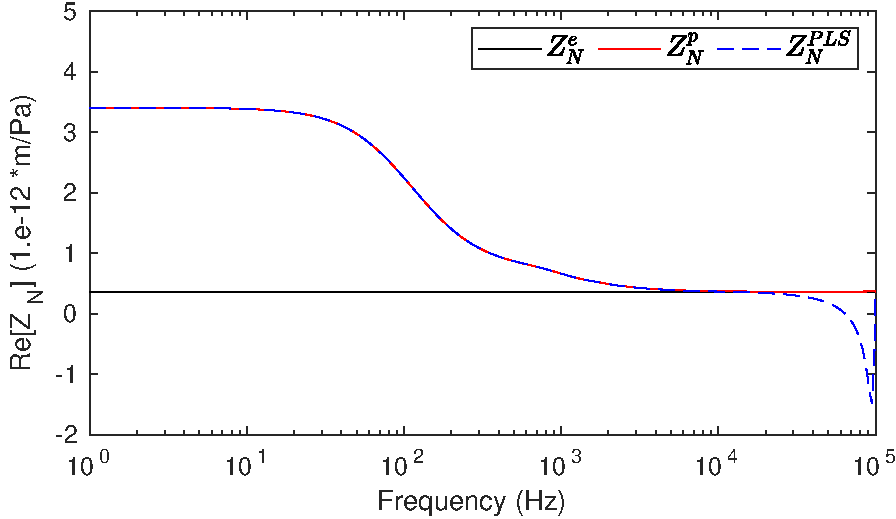
\includegraphics[width=73mm, height=43 mm]{figures/Zn_PLS_compare_1mm_1e-1d.pdf}
%         %\label{}
%         }
%     \subcaptionbox{}
%       {
%         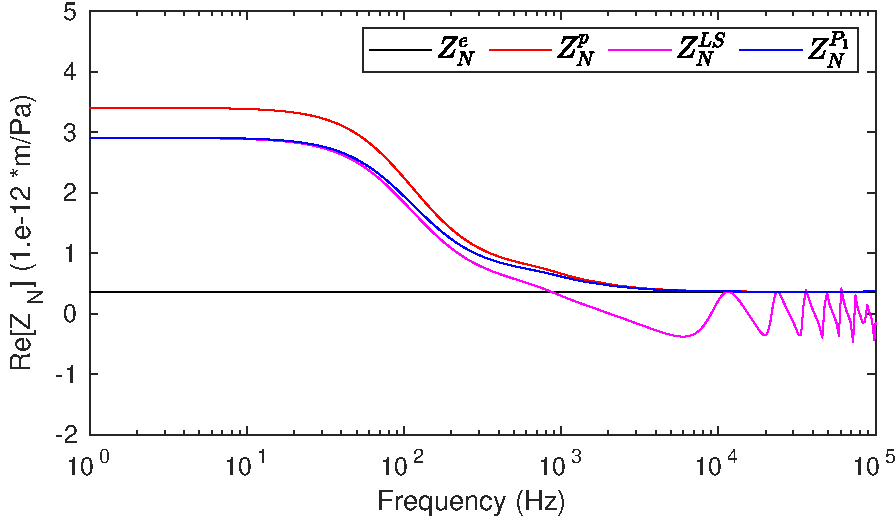
\includegraphics[width=73mm, height=43mm]{figures/Zn_compare_1mm_1e-1d.pdf}
%         %\label{}
%         }
% \caption {Comparison of different estimates of fracture compliance $Z_N$ for the reference properties according table \ref{table:1}.  }
% \label{fig:11}
% \end{figure}


\section{Conclusions}

Our results show that FPD between a fracture and its adjacent DZ increases fracture normal compliance as FPD allows fluid pressure release from the fracture into the DZ.
As a consequence, the reflectivity of the system also increases compared to an impermeable reference model. 
Our results also show that the maximum  increase of normal compliance  and reflectivity are most sensitve to the increse in DZ thickness and porosity as well as to to the decrease of fracture mechanical moduli. In contrast, permeability of the DZ does not have any effect in the maximum increase of reflectivity but controls the transition frequency between FPD regimes and, therefore, constrains the visibility of the FPD effects on reflectivity: the greater the permeability of the DZ, the higher the transition frequency to the unreleaxed FPD regime is, which allows a higher range of frequencies for FPD to contribute in its relaxed regime. The thickness and porosity of the DZ affects both the maximum increase of reflectivity and the transition frequency. Greater thicknesses and porosities increase the reflectivity of the system but shift the transition frequency to lower values. The consequence of this latter is that the visibility of FPD effects on  reflectivity is constrained to lower frequency bands. In this regard, the increase of the DZ thickness and porosity has an opposing effect to that of the increase of the DZ permeability.
Regarding the effect of decreasing the moduli of the DZ, results shown that this decrease limits to lower values the maximum increase of reflectivity due to FPD. However, this effect is counteracted by a likely increase of DZ porosity.
Overall, this study shows that FPD effects promoted by the presence of a DZ in an otherwise impermeable background can enhance the reflectivity of a fracture in the seismic frequency band.




%Text here ===>>>


%%

%  Numbered lines in equations:
%  To add line numbers to lines in equations,
%  \begin{linenomath*}
%  \begin{equation}
%  \end{equation}
%  \end{linenomath*}



%% Enter Figures and Tables near as possible to where they are first mentioned:
%
% DO NOT USE \psfrag or \subfigure commands.
%
% Figure captions go below the figure.
% Table titles go above tables;  other caption information
%  should be placed in last line of the table, using
% \multicolumn2l{$^a$ This is a table note.}
%
%----------------
% EXAMPLE FIGURES
%
% \begin{figure}
% \includegraphics{example.png}
% \caption{caption}
% \end{figure}
%
% Giving latex a width will help it to scale the figure properly. A simple trick is to use \textwidth. Try this if large figures run off the side of the page.
% \begin{figure}
% \noindent\includegraphics[width=\textwidth]{anothersample.png}
%\caption{caption}
%\label{pngfiguresample}
%\end{figure}
%
%
% If you get an error about an unknown bounding box, try specifying the width and height of the figure with the natwidth and natheight options. This is common when trying to add a PDF figure without pdflatex.
% \begin{figure}
% \noindent\includegraphics[natwidth=800px,natheight=600px]{samplefigure.pdf}
%\caption{caption}
%\label{pdffiguresample}
%\end{figure}
%
%
% PDFLatex does not seem to be able to process EPS figures. You may want to try the epstopdf package.
%

%
% ---------------
% EXAMPLE TABLE
%
% \begin{table}
% \caption{Time of the Transition Between Phase 1 and Phase 2$^{a}$}
% \centering
% \begin{tabular}{l c}
% \hline
%  Run  & Time (min)  \\
% \hline
%   $l1$  & 260   \\
%   $l2$  & 300   \\
%   $l3$  & 340   \\
%   $h1$  & 270   \\
%   $h2$  & 250   \\
%   $h3$  & 380   \\
%   $r1$  & 370   \\
%   $r2$  & 390   \\
% \hline
% \multicolumn{2}{l}{$^{a}$Footnote text here.}
% \end{tabular}
% \end{table}

%% SIDEWAYS FIGURE and TABLE
% AGU prefers the use of {sidewaystable} over {landscapetable} as it causes fewer problems.
%
% \begin{sidewaysfigure}
% \includegraphics[width=20pc]{figsamp}
% \caption{caption here}
% \label{newfig}
% \end{sidewaysfigure}
%
%  \begin{sidewaystable}
%  \caption{Caption here}
% \label{tab:signif_gap_clos}
%  \begin{tabular}{ccc}
% one&two&three\\
% four&five&six
%  \end{tabular}
%  \end{sidewaystable}

%% If using numbered lines, please surround equations with \begin{linenomath*}...\end{linenomath*}
%\begin{linenomath*}
%\begin{equation}
%y|{f} \sim g(m, \sigma),
%\end{equation}
%\end{linenomath*}

%%% End of body of article

%%%%%%%%%%%%%%%%%%%%%%%%%%%%%%%%
%% Optional Appendix goes here
%
% The \appendix command resets counters and redefines section heads
%
% After typing \appendix
%
%\section{Here Is Appendix Title}
% will show
% A: Here Is Appendix Title
%
%\appendix
%\section{Here is a sample appendix}

%%%%%%%%%%%%%%%%%%%%%%%%%%%%%%%%%%%%%%%%%%%%%%%%%%%%%%%%%%%%%%%%
%
% Optional Glossary, Notation or Acronym section goes here:
%
%%%%%%%%%%%%%%
% Glossary is only allowed in Reviews of Geophysics
%  \begin{glossary}
%  \term{Term}
%   Term Definition here
%  \term{Term}
%   Term Definition here
%  \term{Term}
%   Term Definition here
%  \end{glossary}

%
%%%%%%%%%%%%%%
% Acronyms
%   \begin{acronyms}
%   \acro{Acronym}
%   Definition here
%   \acro{EMOS}
%   Ensemble model output statistics
%   \acro{ECMWF}
%   Centre for Medium-Range Weather Forecasts
%   \end{acronyms}

%
%%%%%%%%%%%%%%
% Notation
%   \begin{notation}
%   \notation{$a+b$} Notation Definition here
%   \notation{$e=mc^2$}
%   Equation in German-born physicist Albert Einstein's theory of special
%  relativity that showed that the increased relativistic mass ($m$) of a
%  body comes from the energy of motion of the body—that is, its kinetic
%  energy ($E$)—divided by the speed of light squared ($c^2$).
%   \end{notation}




%%%%%%%%%%%%%%%%%%%%%%%%%%%%%%%%%%%%%%%%%%%%%%%%%%%%%%%%%%%%%%%%
%
%  ACKNOWLEDGMENTS
%
% The acknowledgments must list:
%
% >>>>	A statement that indicates to the reader where the data
% 	supporting the conclusions can be obtained (for example, in the
% 	references, tables, supporting information, and other databases).
%
% 	All funding sources related to this work from all authors
%
% 	Any real or perceived financial conflicts of interests for any
%	author
%
% 	Other affiliations for any author that may be perceived as
% 	having a conflict of interest with respect to the results of this
% 	paper.
%
%
% It is also the appropriate place to thank colleagues and other contributors.
% AGU does not normally allow dedications.

\acknowledgments
Enter acknowledgments, including your data availability statement, here.


%% ------------------------------------------------------------------------ %%
%% References and Citations

%%%%%%%%%%%%%%%%%%%%%%%%%%%%%%%%%%%%%%%%%%%%%%%
%
% \bibliography{<name of your .bib file>} don't specify the file extension
%
% don't specify bibliographystyle
%%%%%%%%%%%%%%%%%%%%%%%%%%%%%%%%%%%%%%%%%%%%%%%

\bibliography{reference}
%Reference citation instructions and examples:
%
% Please use ONLY \cite and \citeA for reference citations.
% \cite for parenthetical references
% ...as shown in recent studies (Simpson et al., 2019)
% \citeA for in-text citations
% ...Simpson et al. (2019) have shown...
%
%
%...as shown by \citeA{jskilby}.
%...as shown by \citeA{lewin76}, \citeA{carson86}, \citeA{bartoldy02}, and \citeA{rinaldi03}.
%...has been shown \cite{jskilbye}.
%...has been shown \cite{lewin76,carson86,bartoldy02,rinaldi03}.
%... \cite <i.e.>[]{lewin76,carson86,bartoldy02,rinaldi03}.
%...has been shown by \cite <e.g.,>[and others]{lewin76}.
%
% apacite uses < > for prenotes and [ ] for postnotes
% DO NOT use other cite commands (e.g., \citet, \citep, \citeyear, \nocite, \citealp, etc.).
%
\end{document}



More Information and Advice:

%% ------------------------------------------------------------------------ %%
%
%  SECTION HEADS
%
%% ------------------------------------------------------------------------ %%

% Capitalize the first letter of each word (except for
% prepositions, conjunctions, and articles that are
% three or fewer letters).

% AGU follows standard outline style; therefore, there cannot be a section 1 without
% a section 2, or a section 2.3.1 without a section 2.3.2.
% Please make sure your section numbers are balanced.
% ---------------
% Level 1 head
%
% Use the \section{} command to identify level 1 heads;
% type the appropriate head wording between the curly
% brackets, as shown below.
%
%An example:
%\section{Level 1 Head: Introduction}
%
% ---------------
% Level 2 head
%
% Use the \subsection{} command to identify level 2 heads.
%An example:
%\subsection{Level 2 Head}
%
% ---------------
% Level 3 head
%
% Use the \subsubsection{} command to identify level 3 heads
%An example:
%\subsubsection{Level 3 Head}
%
%---------------
% Level 4 head
%
% Use the \subsubsubsection{} command to identify level 3 heads
% An example:
%\subsubsubsection{Level 4 Head} An example.
%
%% ------------------------------------------------------------------------ %%
%
%  IN-TEXT LISTS
%
%% ------------------------------------------------------------------------ %%
%
% Do not use bulleted lists; enumerated lists are okay.
% \begin{enumerate}
% \item
% \item
% \item
% \end{enumerate}
%
%% ------------------------------------------------------------------------ %%
%
%  EQUATIONS
%
%% ------------------------------------------------------------------------ %%

% Single-line equations are centered.
% Equation arrays will appear left-aligned.

Math coded inside display math mode \[ ...\]
 will not be numbered, e.g.,:
 \[ x^2=y^2 + z^2\]

 Math coded inside \begin{equation} and \end{equation} will
 be automatically numbered, e.g.,:
 \begin{equation}
 x^2=y^2 + z^2
 \end{equation}


% To create multiline equations, use the
% \begin{eqnarray} and \end{eqnarray} environment
% as demonstrated below.
\begin{eqnarray}
  x_{1} & = & (x - x_{0}) \cos \Theta \nonumber \\
        && + (y - y_{0}) \sin \Theta  \nonumber \\
  y_{1} & = & -(x - x_{0}) \sin \Theta \nonumber \\
        && + (y - y_{0}) \cos \Theta.
\end{eqnarray}

%If you don't want an equation number, use the star form:
%\begin{eqnarray*}...\end{eqnarray*}

% Break each line at a sign of operation
% (+, -, etc.) if possible, with the sign of operation
% on the new line.

% Indent second and subsequent lines to align with
% the first character following the equal sign on the
% first line.

% Use an \hspace{} command to insert horizontal space
% into your equation if necessary. Place an appropriate
% unit of measure between the curly braces, e.g.
% \hspace{1in}; you may have to experiment to achieve
% the correct amount of space.


%% ------------------------------------------------------------------------ %%
%
%  EQUATION NUMBERING: COUNTER
%
%% ------------------------------------------------------------------------ %%

% You may change equation numbering by resetting
% the equation counter or by explicitly numbering
% an equation.

% To explicitly number an equation, type \eqnum{}
% (with the desired number between the brackets)
% after the \begin{equation} or \begin{eqnarray}
% command.  The \eqnum{} command will affect only
% the equation it appears with; LaTeX will number
% any equations appearing later in the manuscript
% according to the equation counter.
%

% If you have a multiline equation that needs only
% one equation number, use a \nonumber command in
% front of the double backslashes (\\) as shown in
% the multiline equation above.

% If you are using line numbers, remember to surround
% equations with \begin{linenomath*}...\end{linenomath*}

%  To add line numbers to lines in equations:
%  \begin{linenomath*}
%  \begin{equation}
%  \end{equation}
%  \end{linenomath*}



